\documentclass[12pt]{article}
\usepackage[a4paper, margin=1in]{geometry}
\usepackage{enumitem}
\usepackage{titlesec}
\usepackage{graphicx}
\usepackage{hyperref}
\usepackage{float}
\titleformat{\section}{\Large\bfseries}{\thesection}{1em}{}
\titleformat{\subsection}{\large\bfseries}{\thesubsection}{1em}{}
\title{User Manual\\Taxi Tap by Git It Done}
\date{}
\begin{document}
\maketitle
\begin{figure}[H]
  \centering
  
\includegraphics[width=0.5\textwidth]{LogoGroup.png} 
\end{figure}
\begin{figure}[H]
  \centering
  
\includegraphics[width=0.5\textwidth]{LogoTaxiTap.png} 
\end{figure}
\newpage
\tableofcontents
\newpage

\section{Getting Started}

\subsection{Logging In and Signing Up}

TaxiTap provides separate interfaces for passengers and drivers. To get started, you'll need to create an account or log in to your existing account.

\subsubsection{Sign Up}
To create a new account, you'll need to provide the following information:
\begin{itemize}
    \item Full Name
    \item Phone Number
    \item Password
    \item Role (Passenger or Driver)
\end{itemize}

\begin{figure}[H]
  \centering
  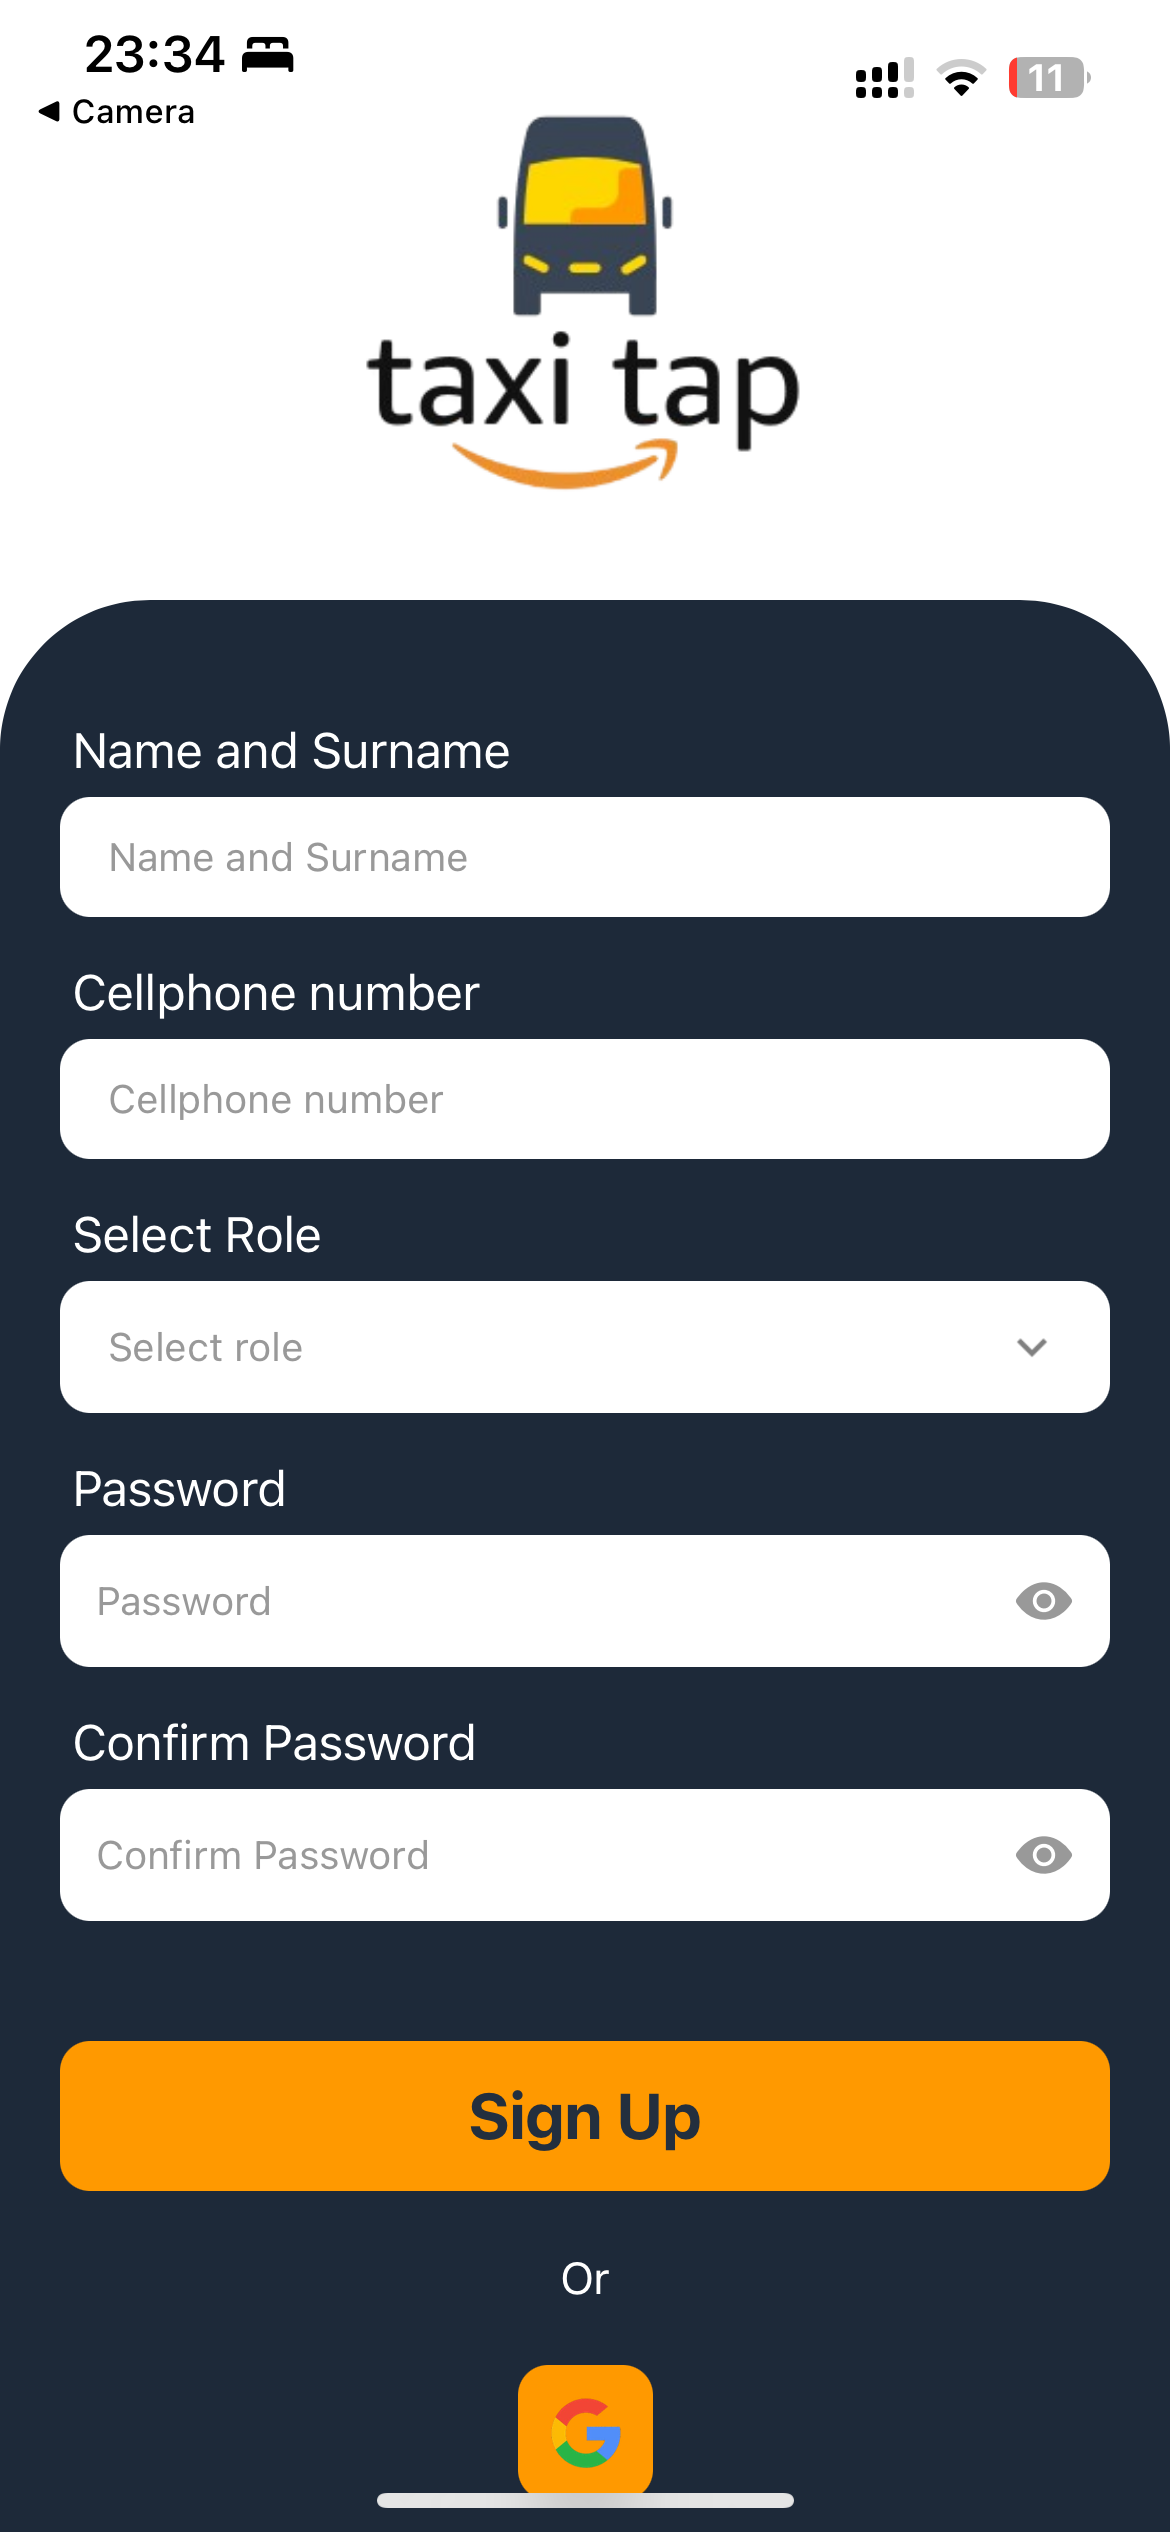
\includegraphics[width=0.4\textwidth]{signup2.png}
  \caption{Sign Up Screen}
\end{figure}

\begin{figure}[H]
  \centering
  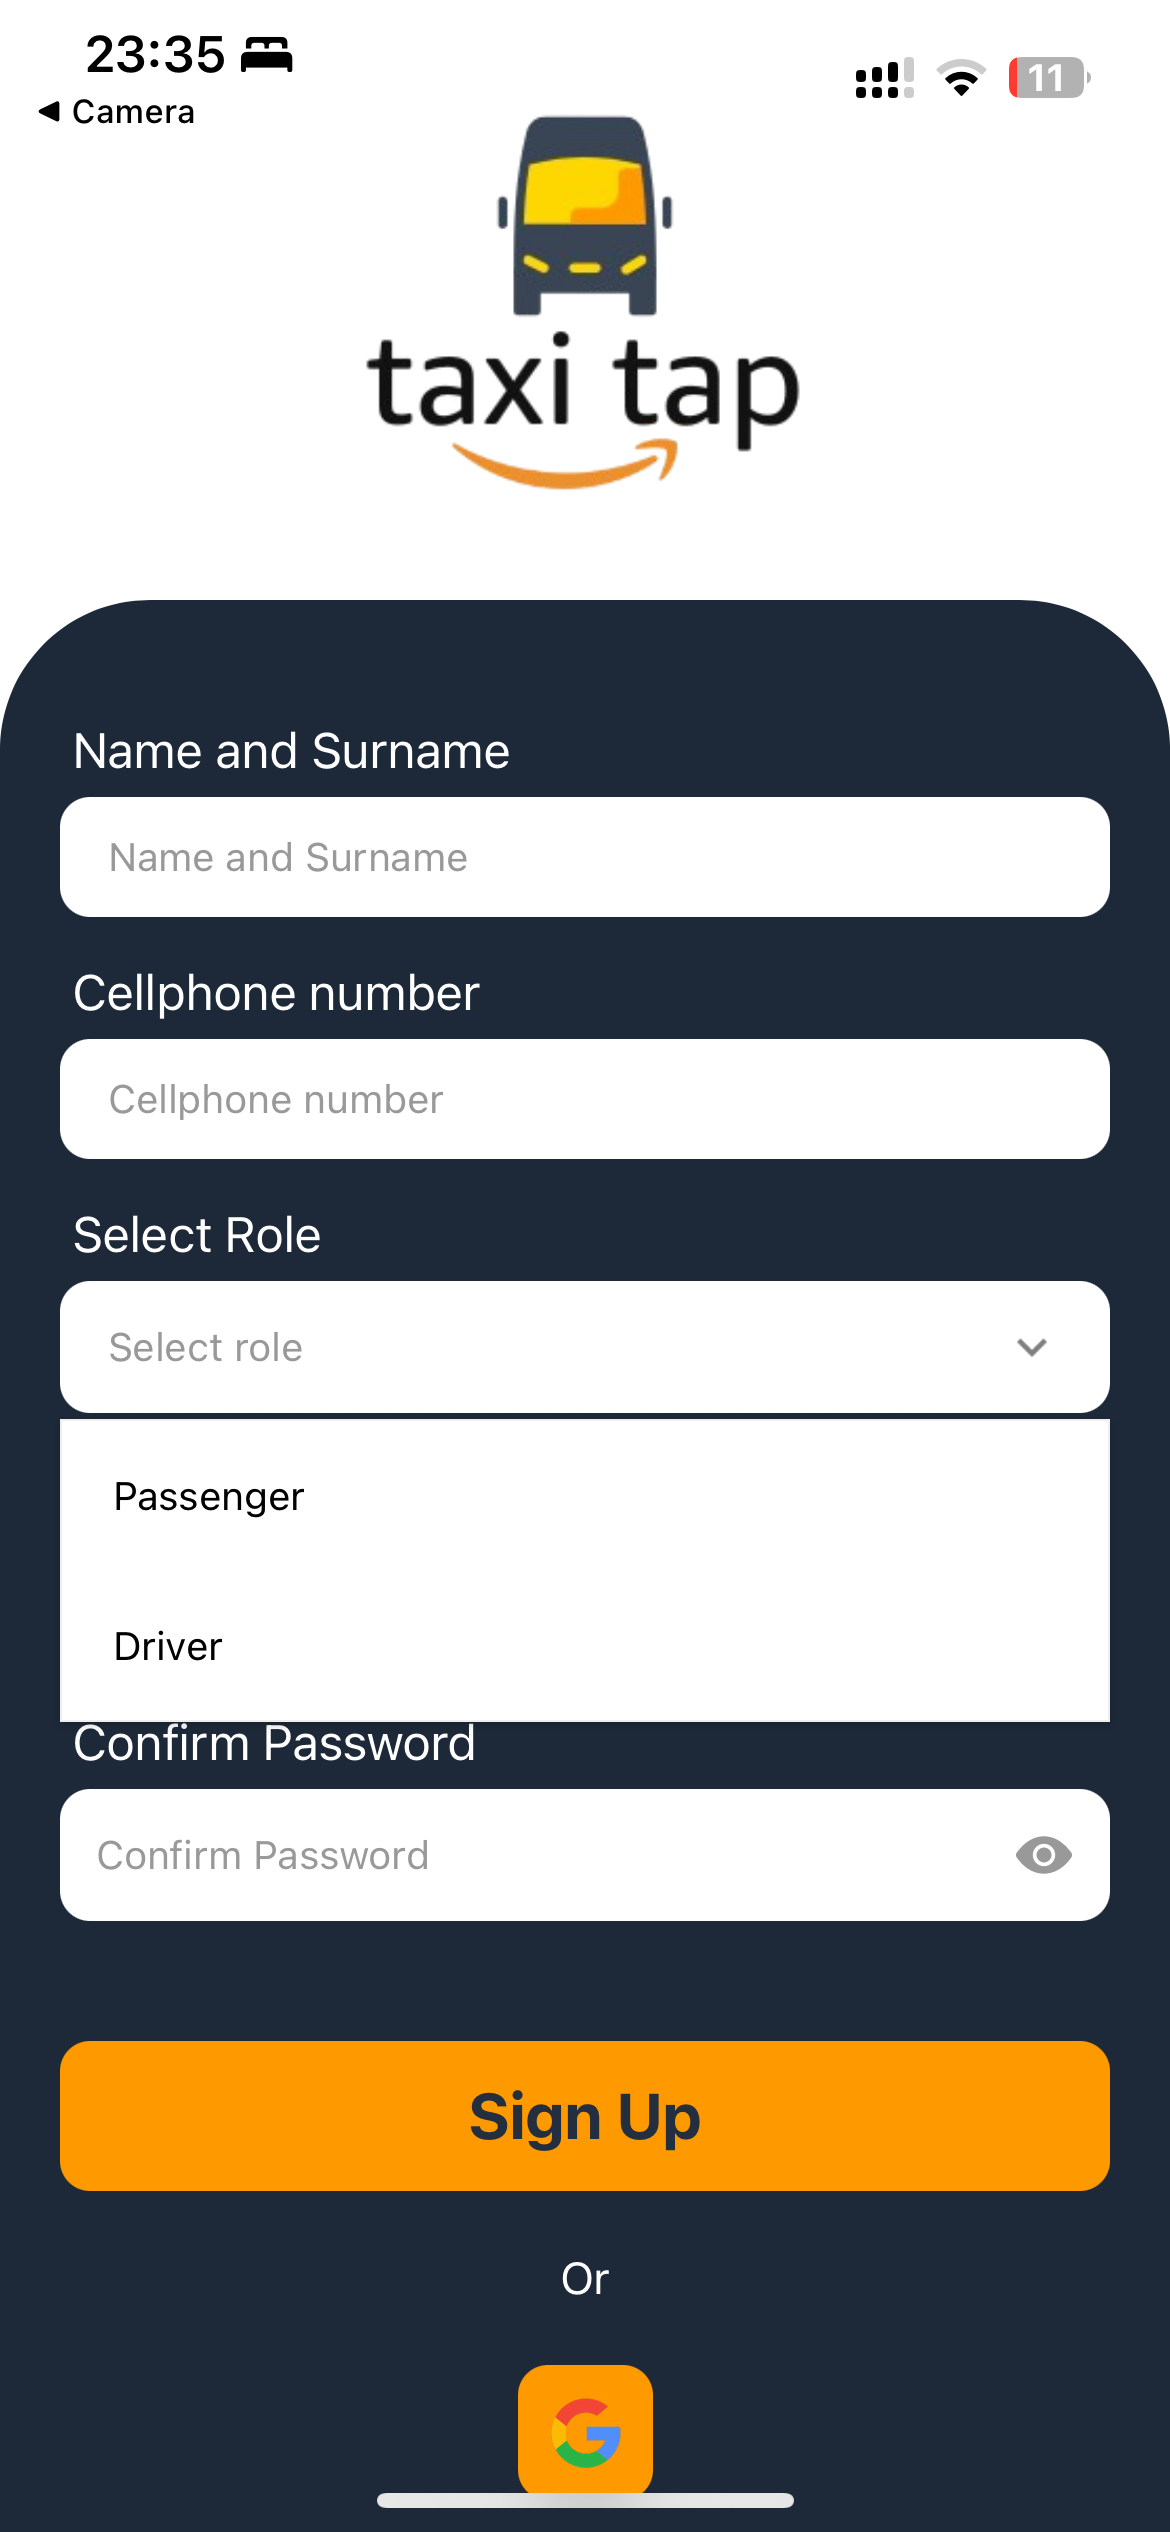
\includegraphics[width=0.4\textwidth]{signup_roles.png}
  \caption{Sign Up Screen}
\end{figure}

\subsubsection{Log In}
To log in to your existing account, you'll need:
\begin{itemize}
    \item Phone Number
    \item Password
\end{itemize}

\begin{figure}[H]
  \centering
  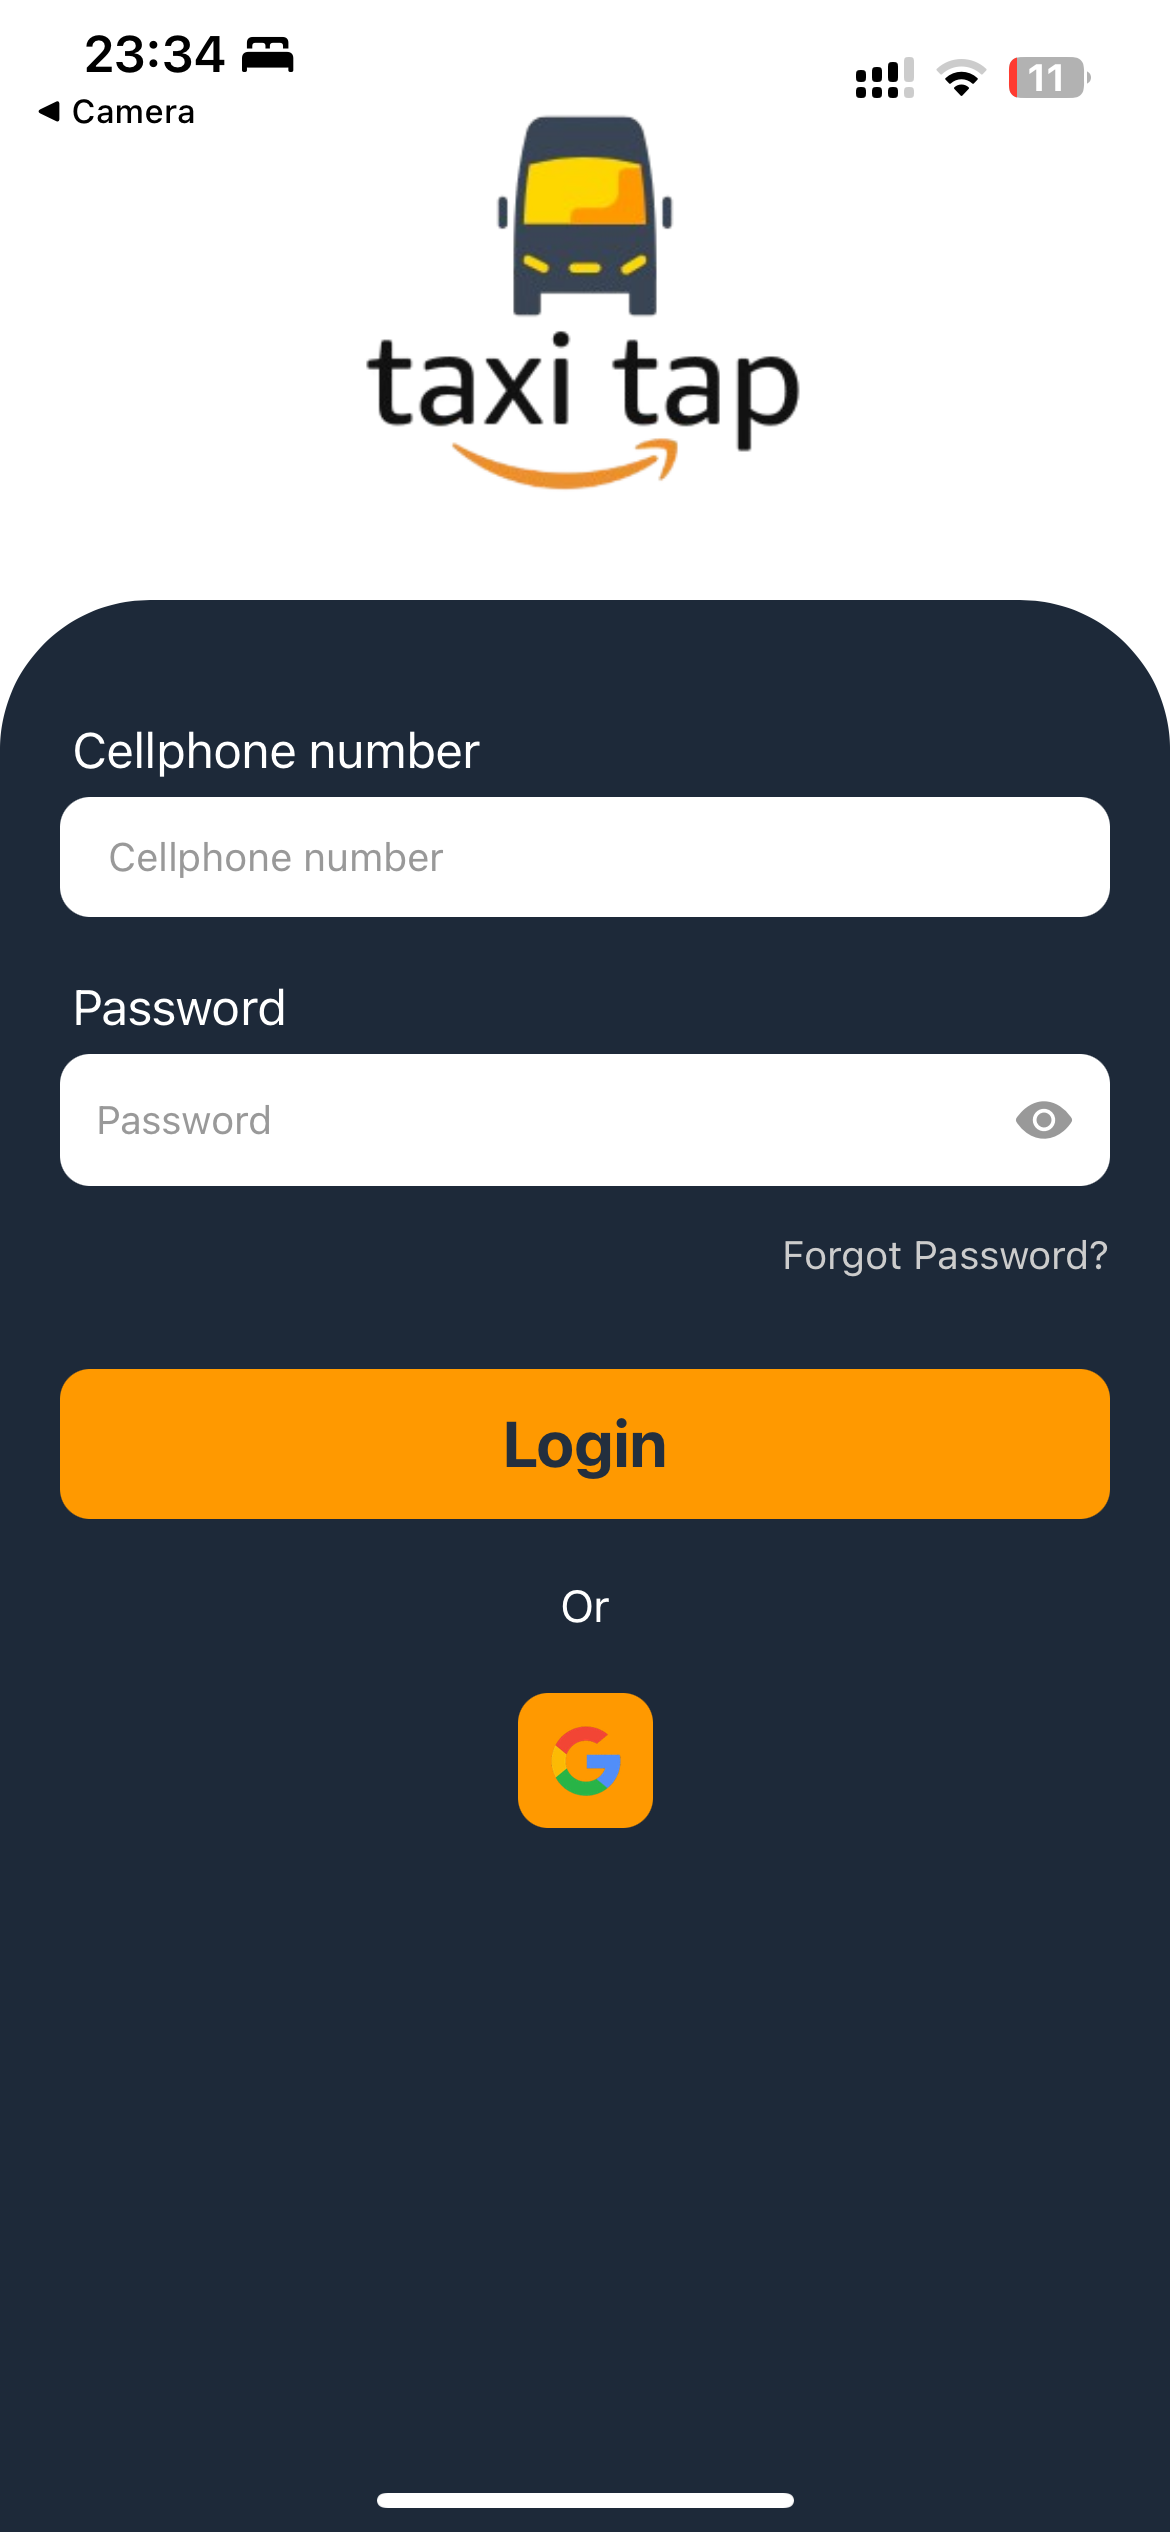
\includegraphics[width=0.6\textwidth]{login2.png}
  \caption{Login Screen}
\end{figure}

\newpage

\section{Passenger Interface}

\subsection{Requesting a Ride}

\subsubsection{Step 1: Enter Destination Details}
\begin{enumerate}
    \item Open the TaxiTap app and ensure you're logged in as a passenger
    \item On the main screen, you'll see a map with your current location
    \item Type in your destination address in the destination field
    \item The system will automatically detect your current location as the origin, or you can manually enter your pickup address
\end{enumerate}

\begin{figure}[H]
  \centering
  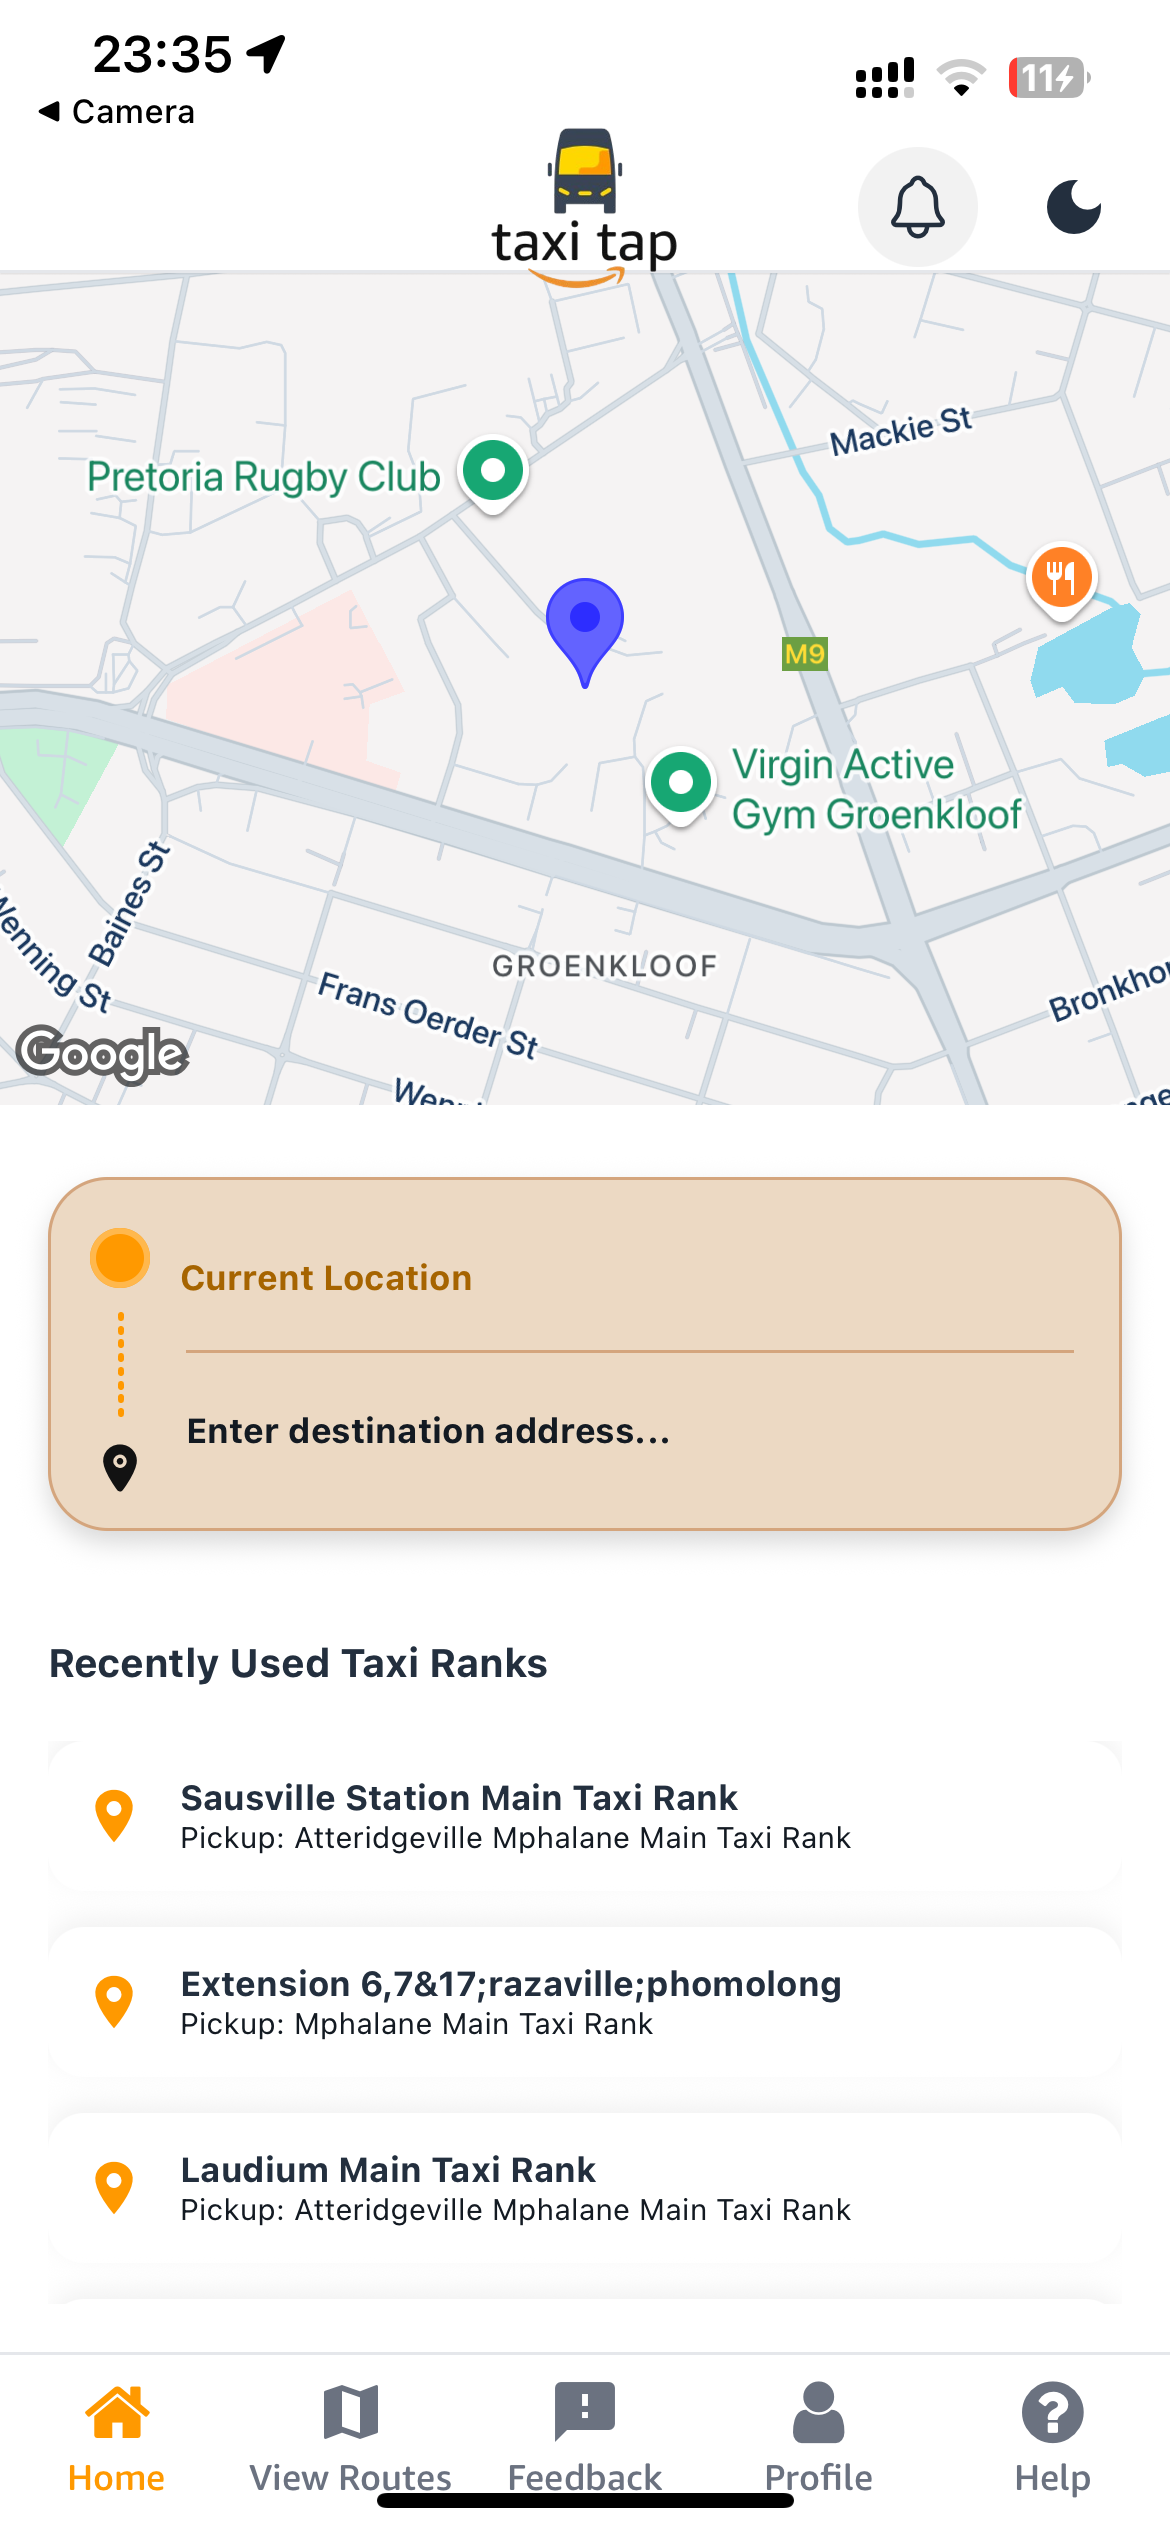
\includegraphics[width=0.4\textwidth]{destination_entry.png}
  \caption{Entering Destination}
\end{figure}

\subsubsection{Step 2: Check for Available Taxis}
The app will search for available taxis that:
\begin{itemize}
    \item Are nearby your location
    \item Follow routes with stops near both your origin and destination
\end{itemize}

If taxis are available, you'll see:
\begin{itemize}
    \item Number of available taxis
    \item Number of matching routes
    \item A "Ready to book your ride!" confirmation message
\end{itemize}

\begin{figure}[H]
  \centering
  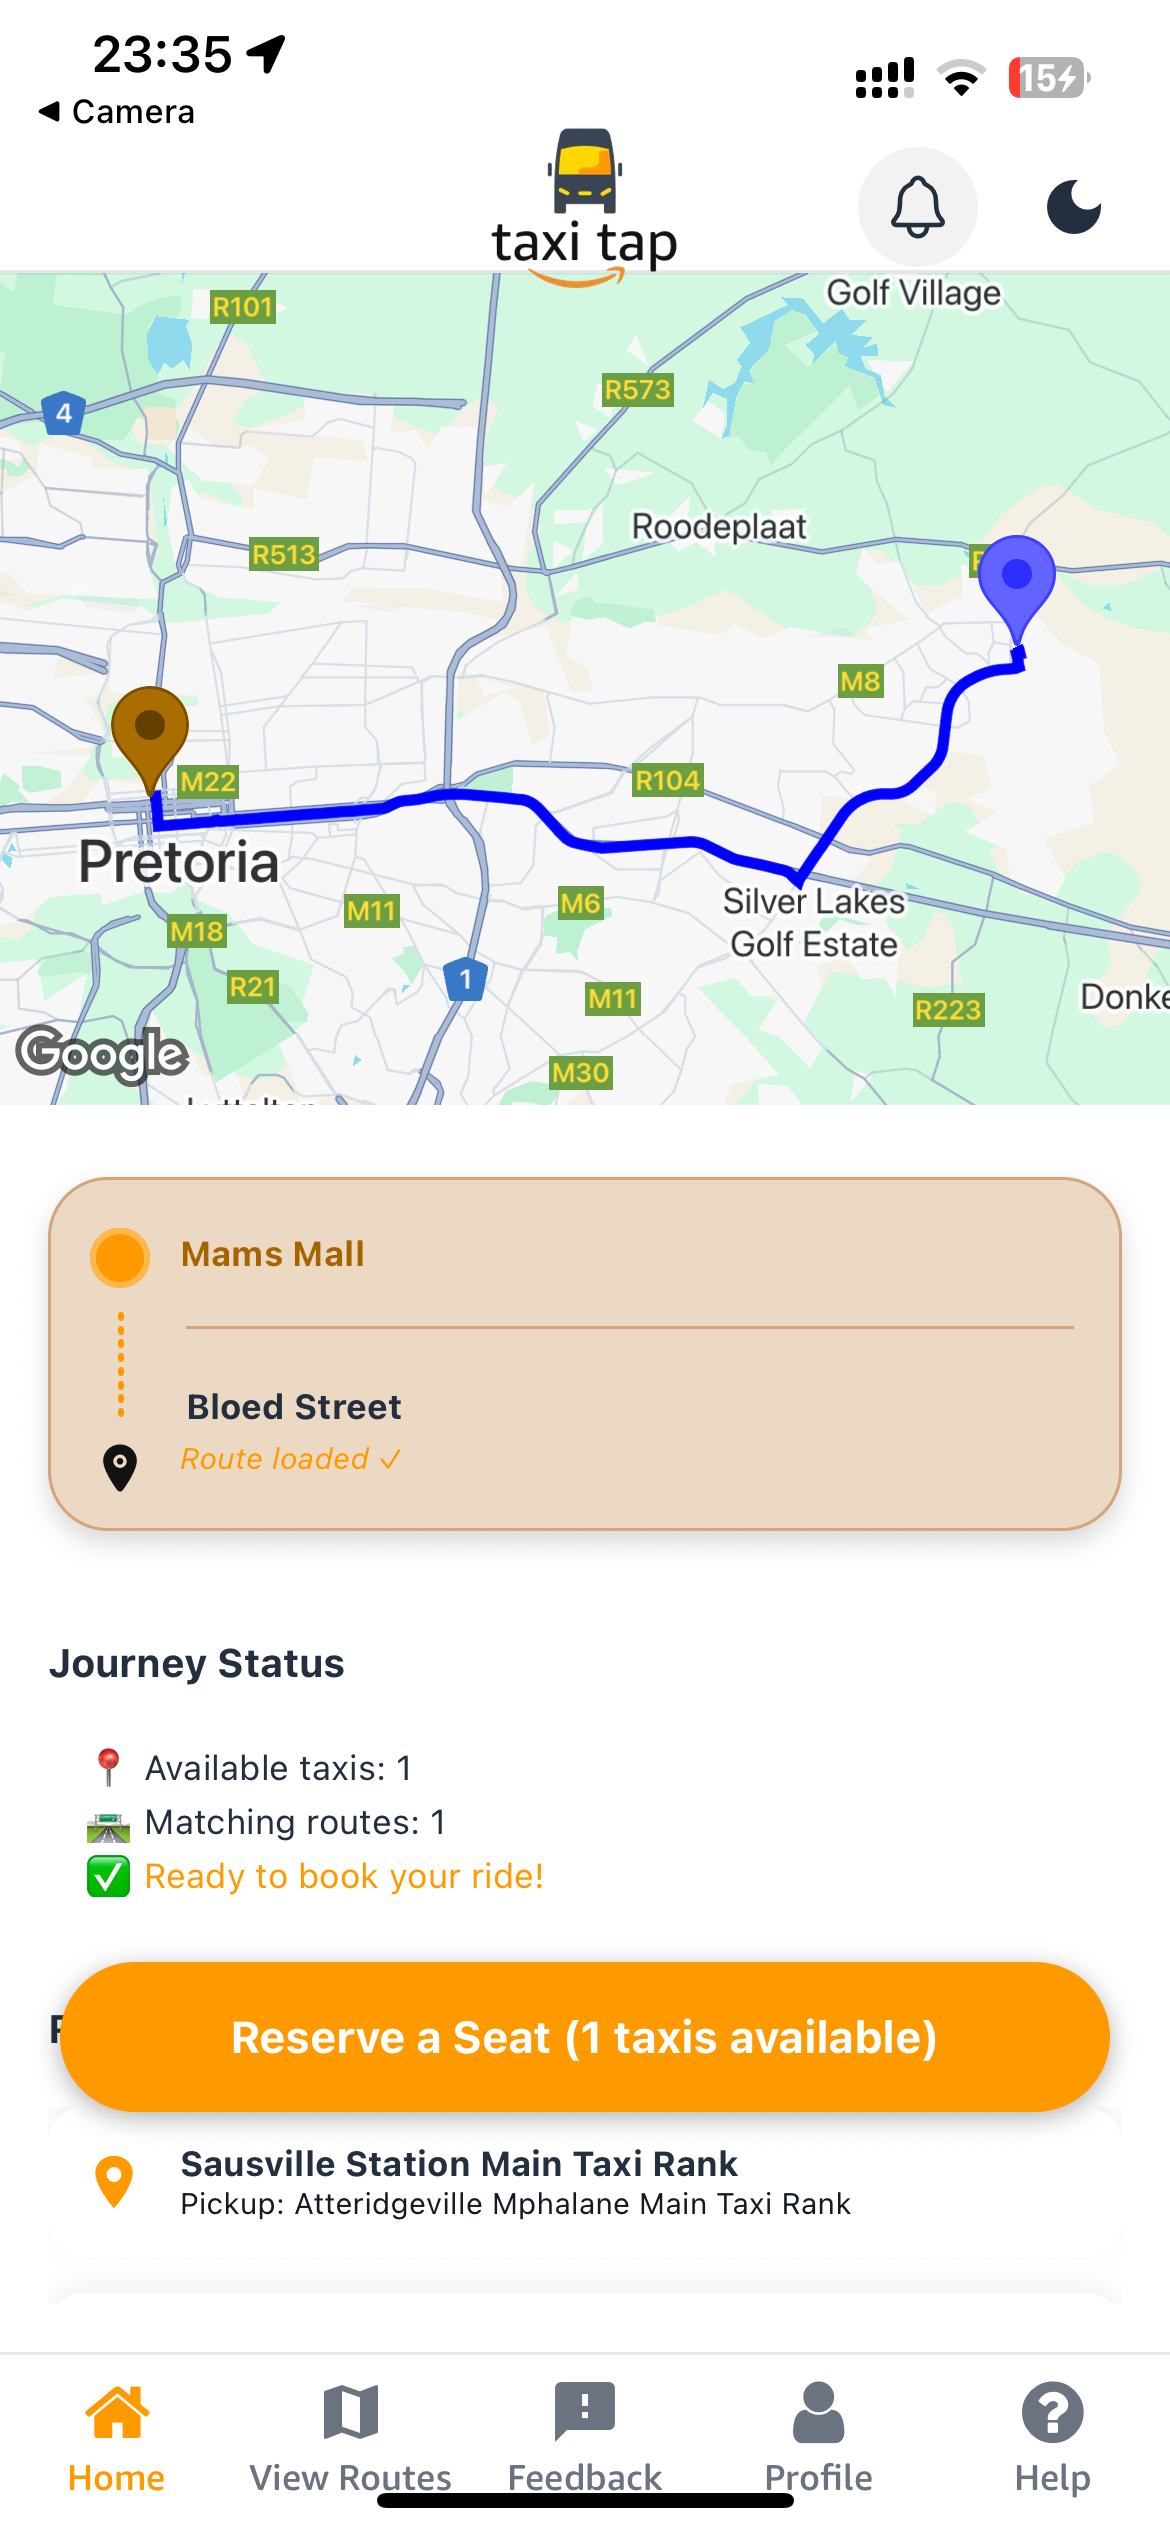
\includegraphics[width=0.4\textwidth]{available_taxis.png}
  \caption{Available Taxis Display}
\end{figure}

\subsubsection{Step 3: Reserve Your Seat}
Once available taxis are found, click the orange "Reserve a Seat" button to proceed to taxi selection.

\subsection{Selecting Your Driver and Taxi}

\subsubsection{Available Taxis Page}
After clicking "Reserve a Seat," you'll be taken to the "Available Taxis" page where you can see:

\begin{itemize}
    \item Driver name and details
    \item Vehicle information (make, model, license plate)
    \item Route information
    \item Estimated fare
    \item Estimated duration
    \item Driver's current distance from you
    \item Driver rating (5-star system)
\end{itemize}

\begin{figure}[H]
  \centering
  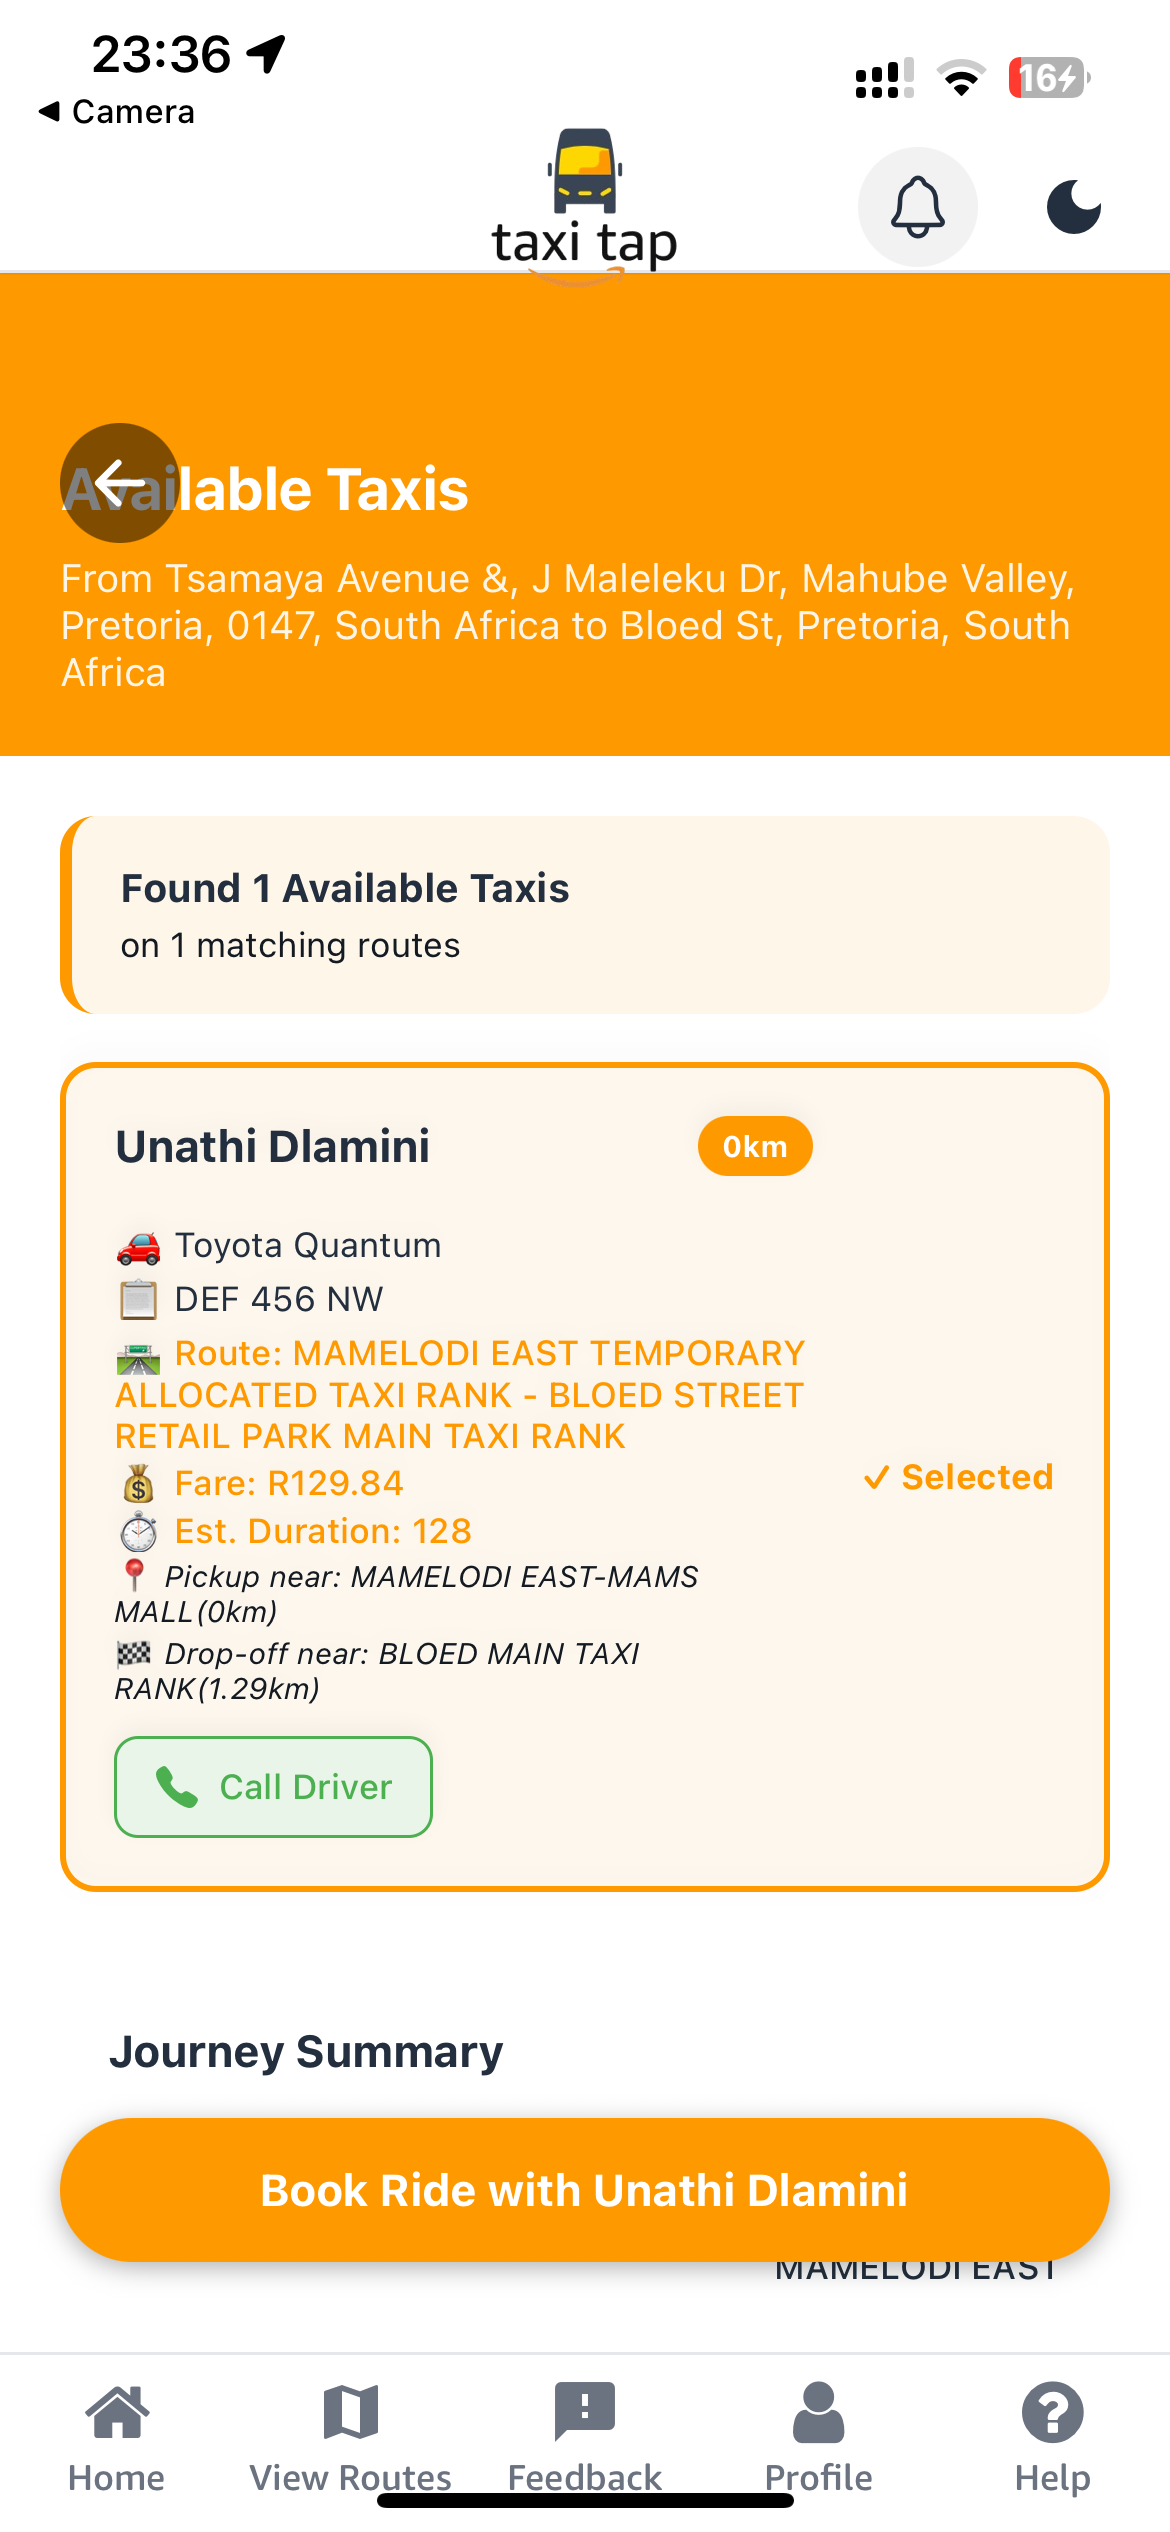
\includegraphics[width=0.4\textwidth]{taxi_selection.png}
  \caption{Taxi Selection Screen}
\end{figure}

\subsubsection{Step 4: Book Your Ride}
\begin{enumerate}
    \item Review the taxi and driver information
    \item Check the fare and estimated duration
    \item Click the orange "Book Ride with [Driver's Name]" button
    \item You can also use the "Call Driver" button to contact the driver directly
\end{enumerate}

\subsection{Managing Your Ride Request}

\subsubsection{Ride Request Sent}
After booking, you'll see a confirmation that your ride request has been sent to the driver. At this stage:
\begin{itemize}
    \item The driver will be notified of your request
    \item You'll receive a notification when the driver responds
    \item You can still cancel the request if needed
\end{itemize}

\begin{figure}[H]
  \centering
  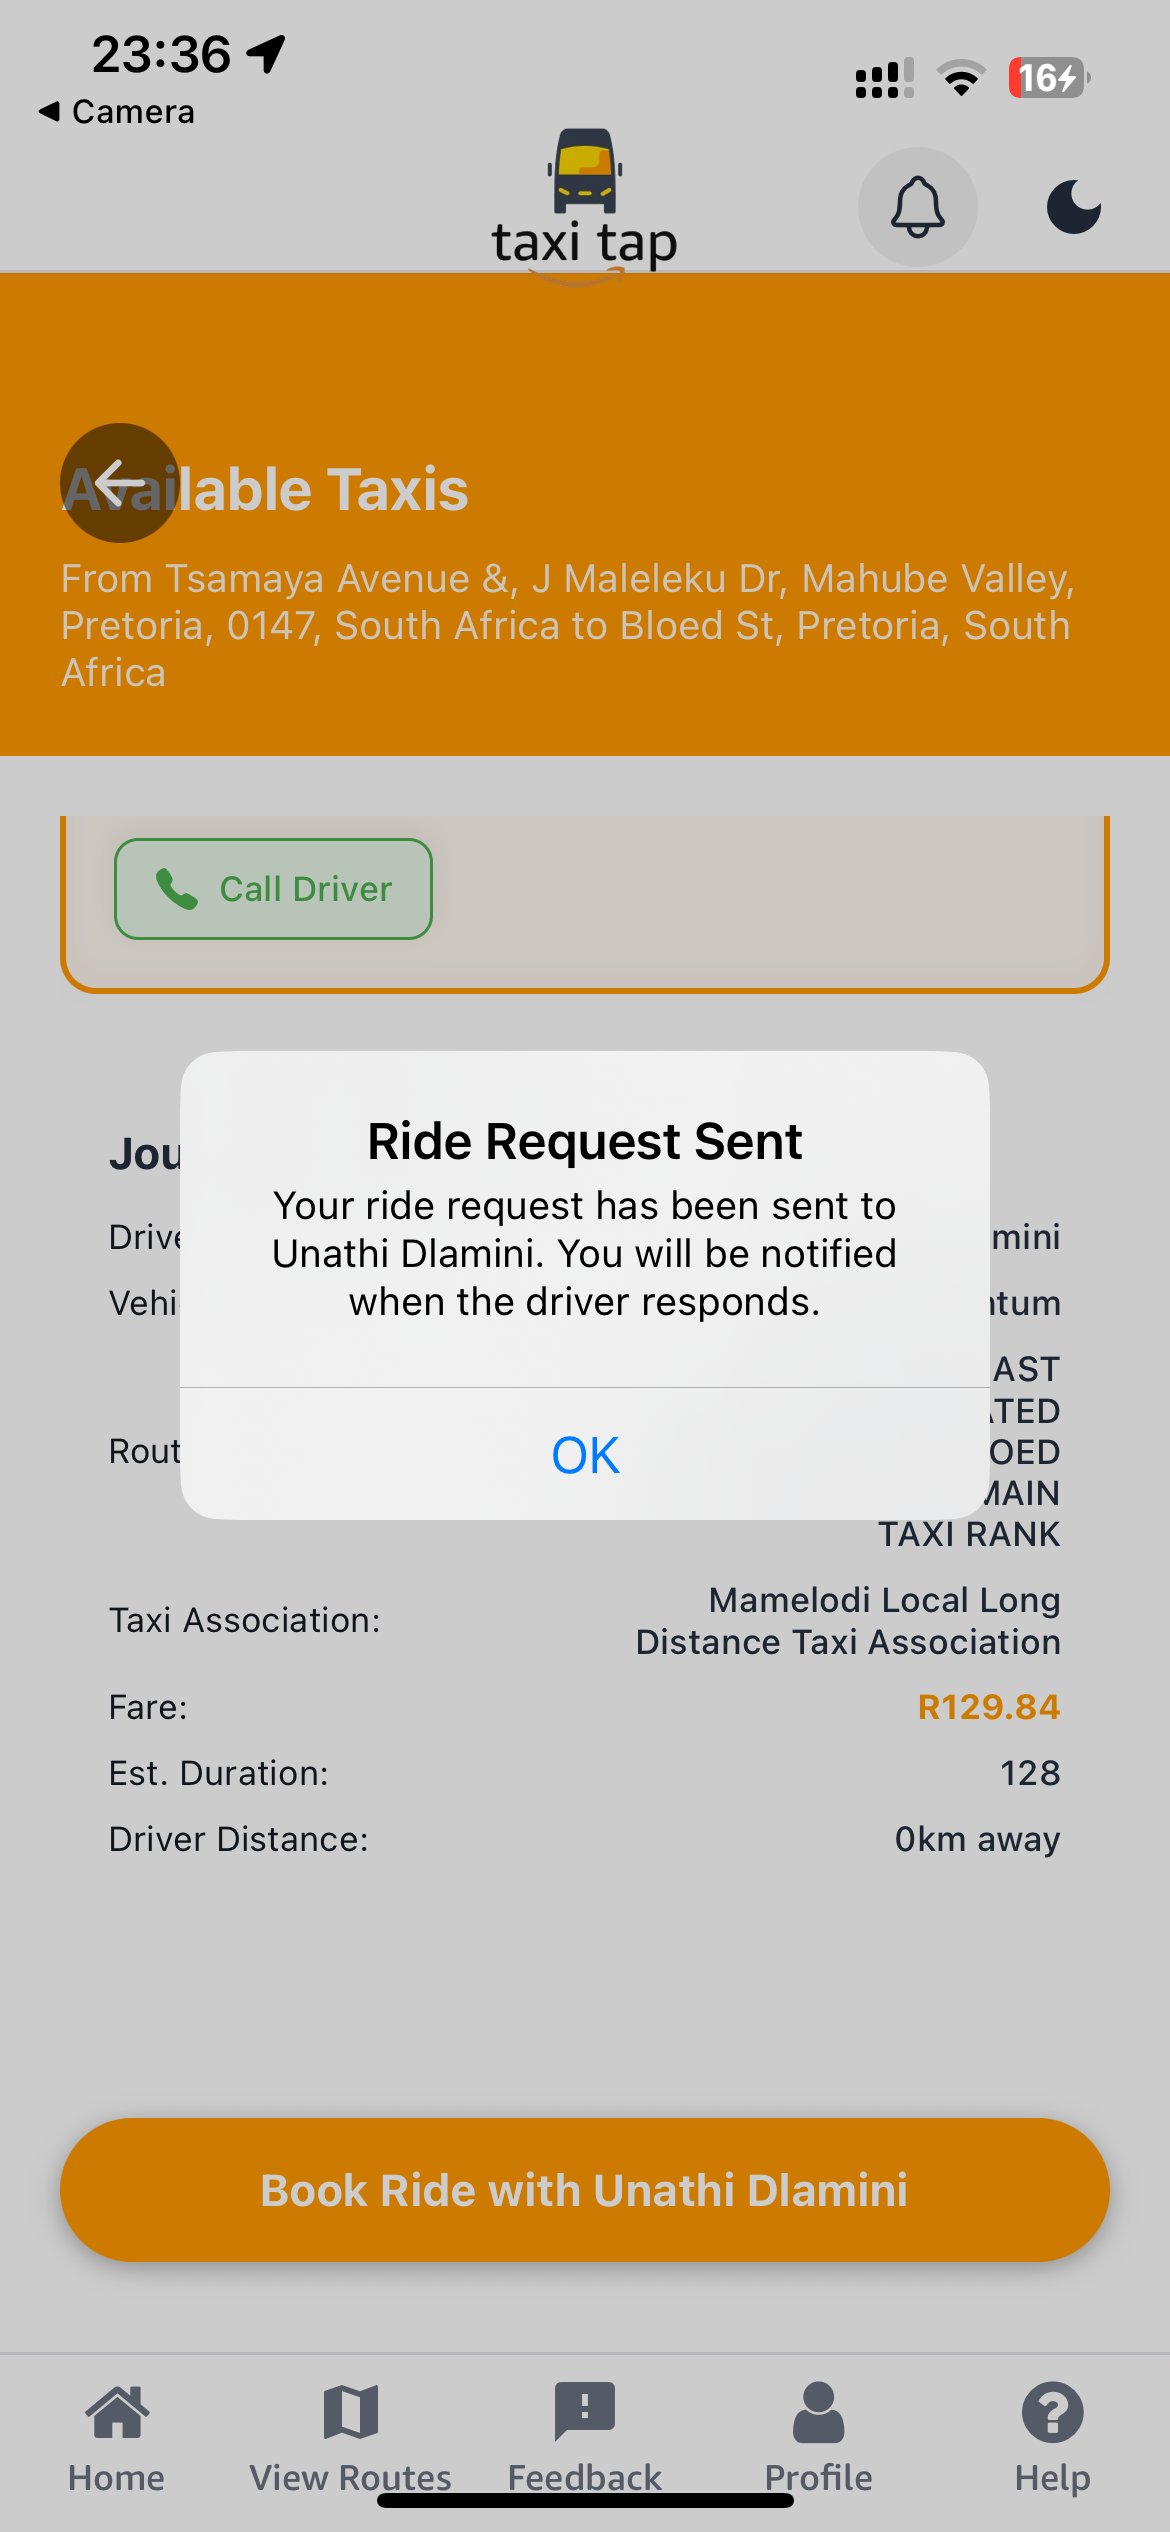
\includegraphics[width=0.4\textwidth]{ride_request_sent.png}
  \caption{Ride Request Sent Confirmation}
\end{figure}

\subsubsection{Ride Accepted}
When the driver accepts your request:
\begin{itemize}
    \item You'll receive a "Ride Accepted" notification
    \item The message will confirm "Your ride has been accepted. Driver is on the way!"
    \item You can track the driver's location on the map
    \item The "Start Ride" button will become available
\end{itemize}

\begin{figure}[H]
  \centering
  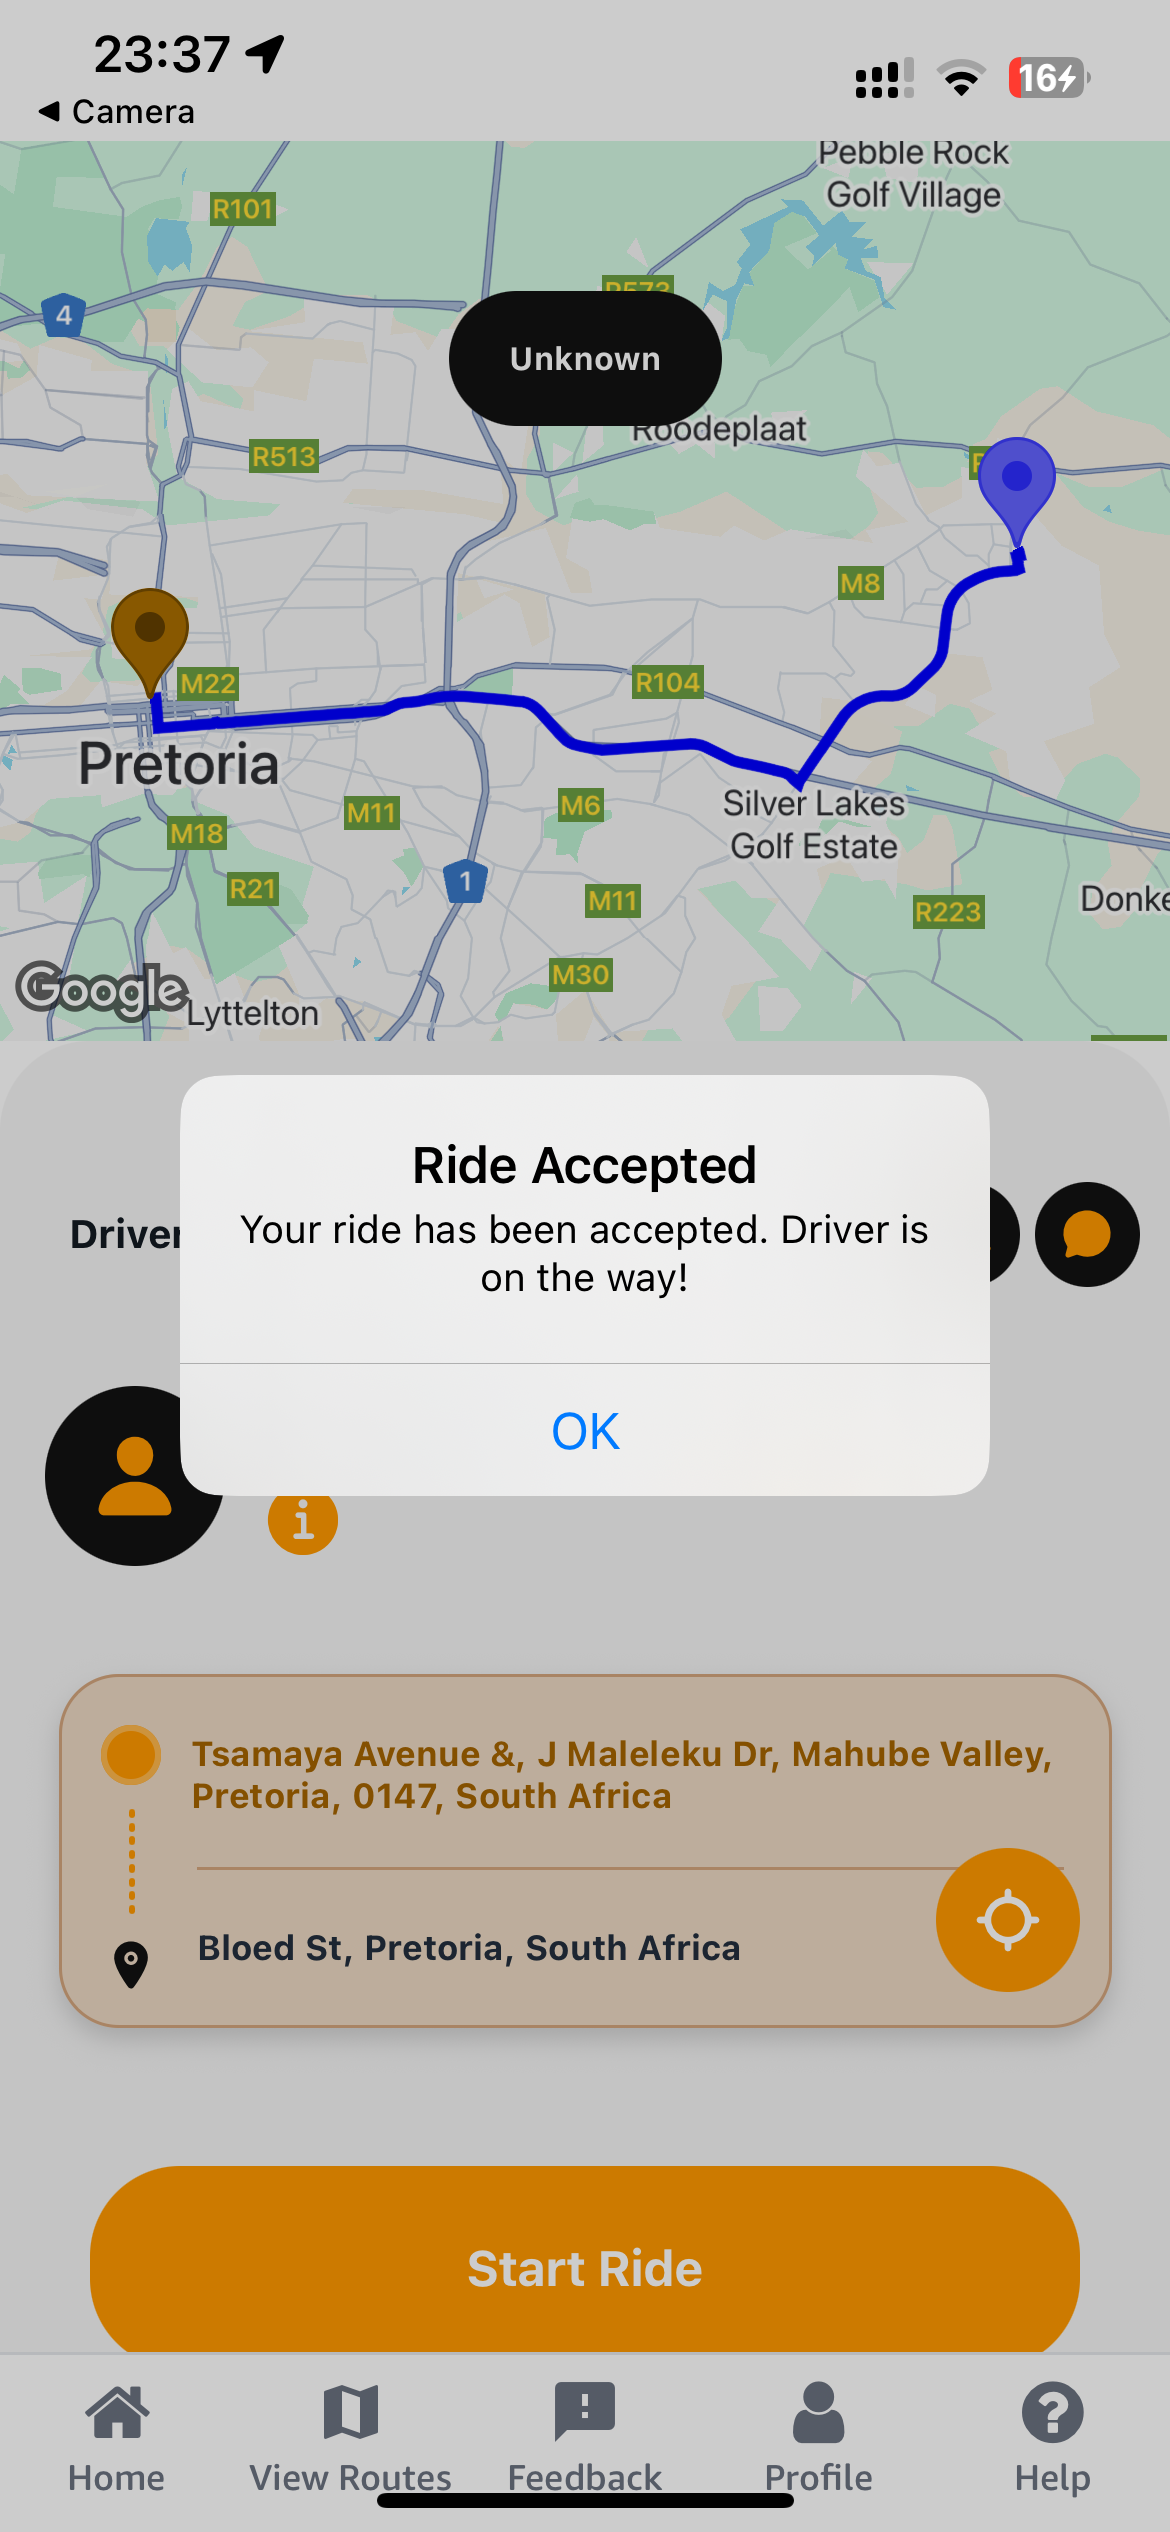
\includegraphics[width=0.4\textwidth]{ride_accepted.png}
  \caption{Ride Accepted Notification}
\end{figure}

\subsection{During the Ride}

\subsubsection{Starting Your Ride}
\begin{enumerate}
    \item When the driver arrives at your pickup location, click "Start Ride"
    \item This confirms that you have boarded the taxi
    \item You'll see a "Ride Started" confirmation message
    \item The app will display "Your ride has started. Enjoy your journey!"
\end{enumerate}

\begin{figure}[H]
  \centering
  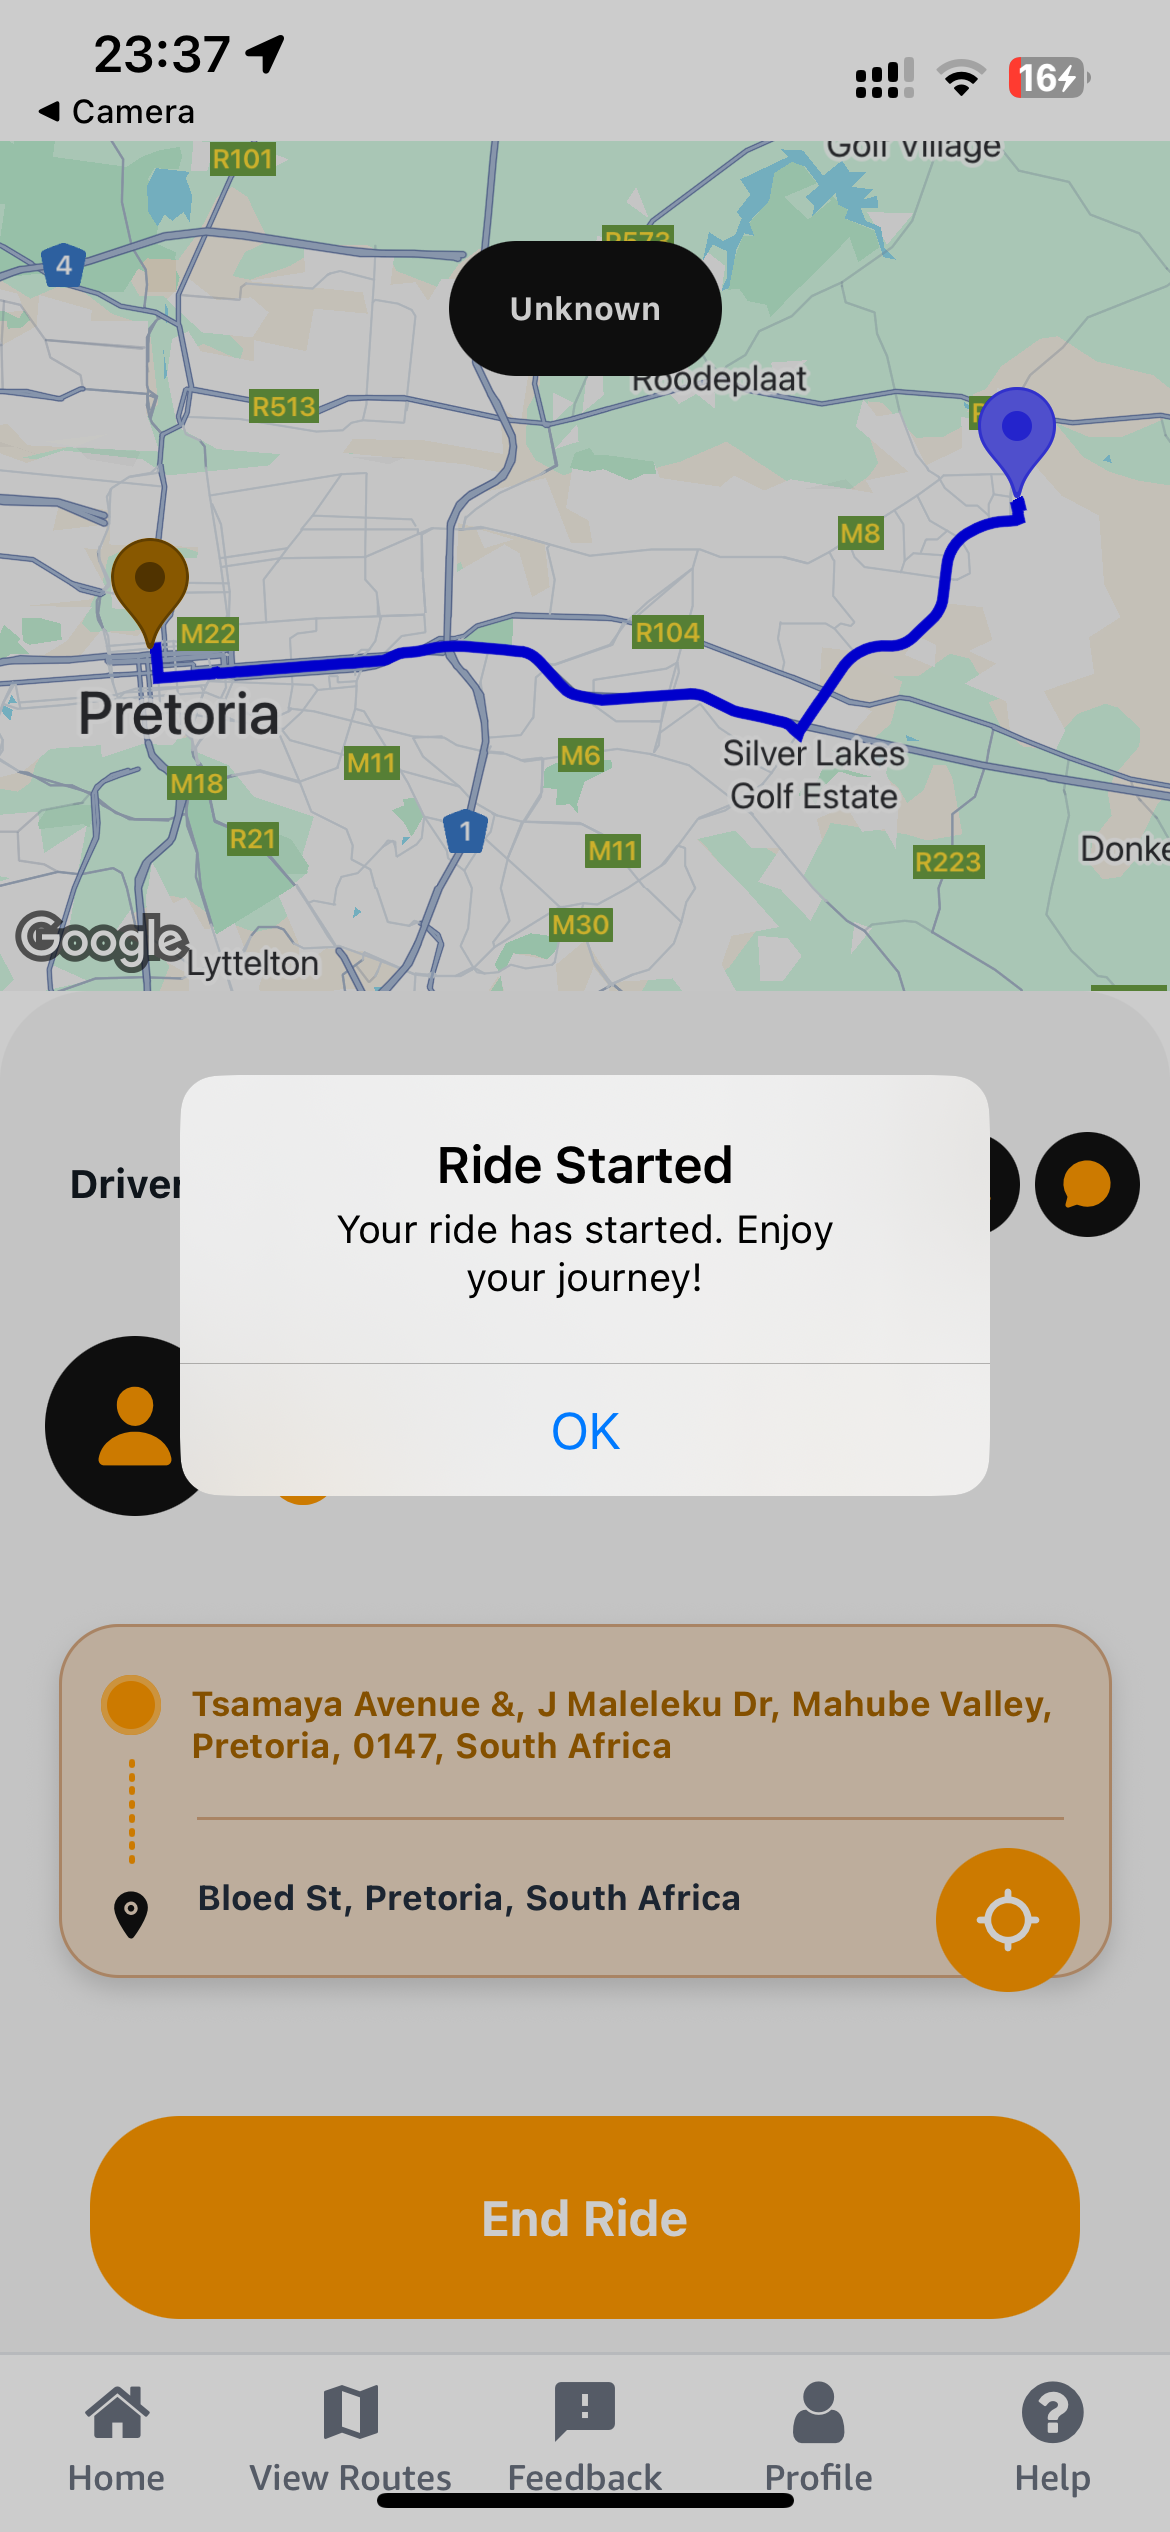
\includegraphics[width=0.4\textwidth]{ride_started.png}
  \caption{Ride Started Confirmation}
\end{figure}

\subsubsection{Ride Tracking}
During your ride, you can:
\begin{itemize}
    \item View your route on the map
    \item See driver details and rating
    \item Access emergency contact options
    \item Monitor your journey progress
\end{itemize}

\begin{figure}[H]
  \centering
  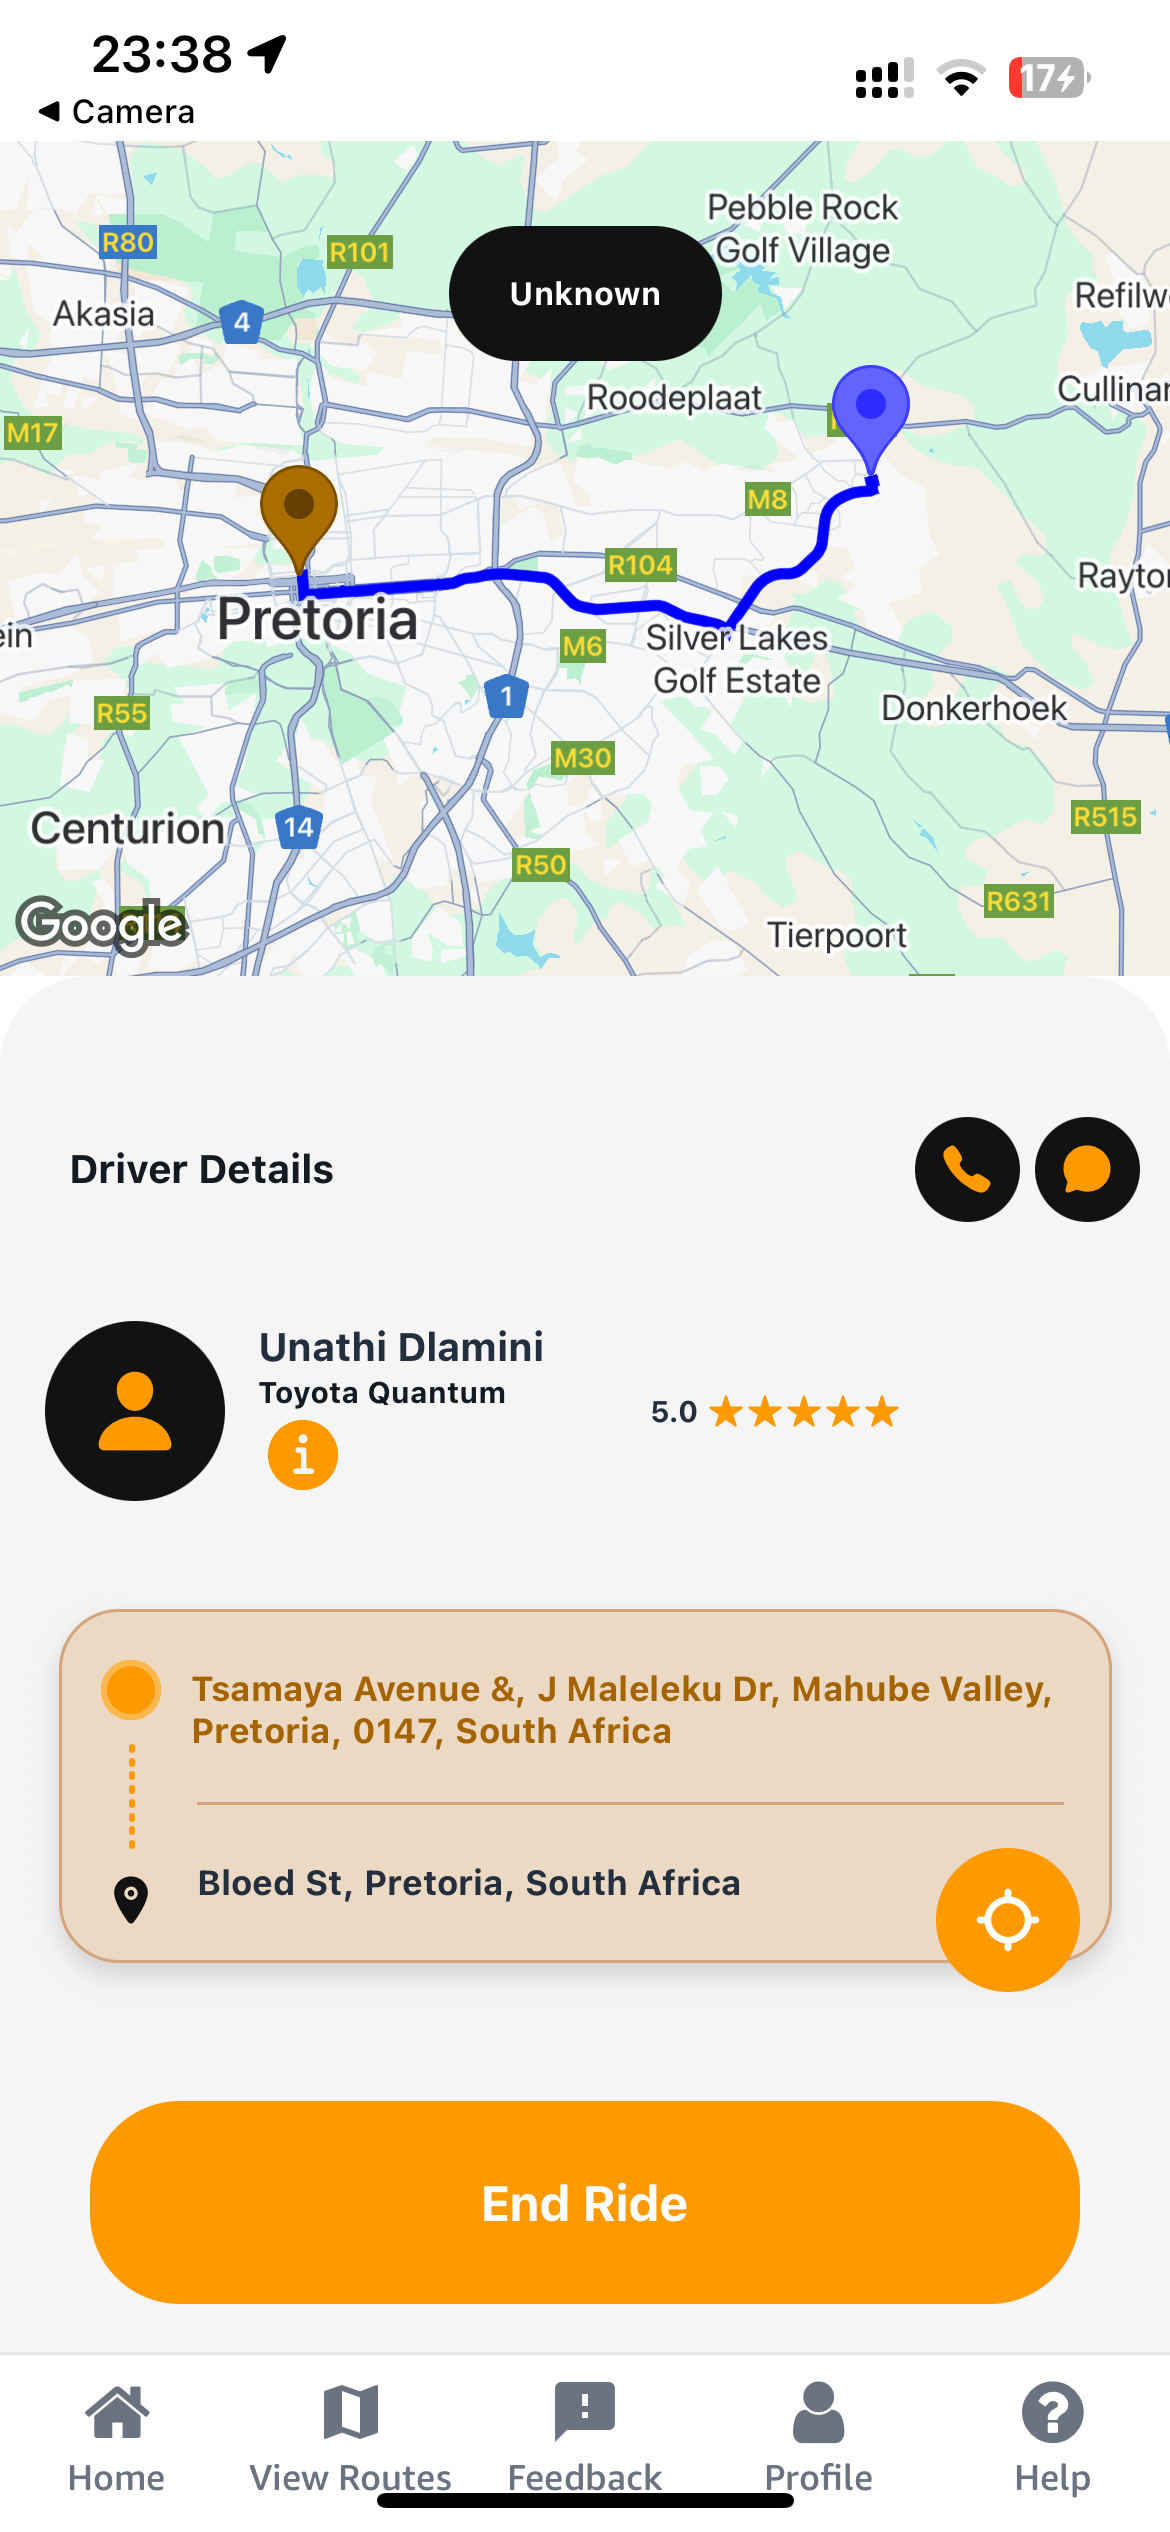
\includegraphics[width=0.4\textwidth]{during_ride.png}
  \caption{During Ride Interface}
\end{figure}

\subsubsection{Ending Your Ride}
\begin{enumerate}
    \item When you reach your destination and are ready to disembark
    \item Click the "End Ride" button
    \item You'll receive a "Success - Ride ended!" confirmation
    \item The app will return to the main screen, ready for your next journey
\end{enumerate}

\begin{figure}[H]
  \centering
  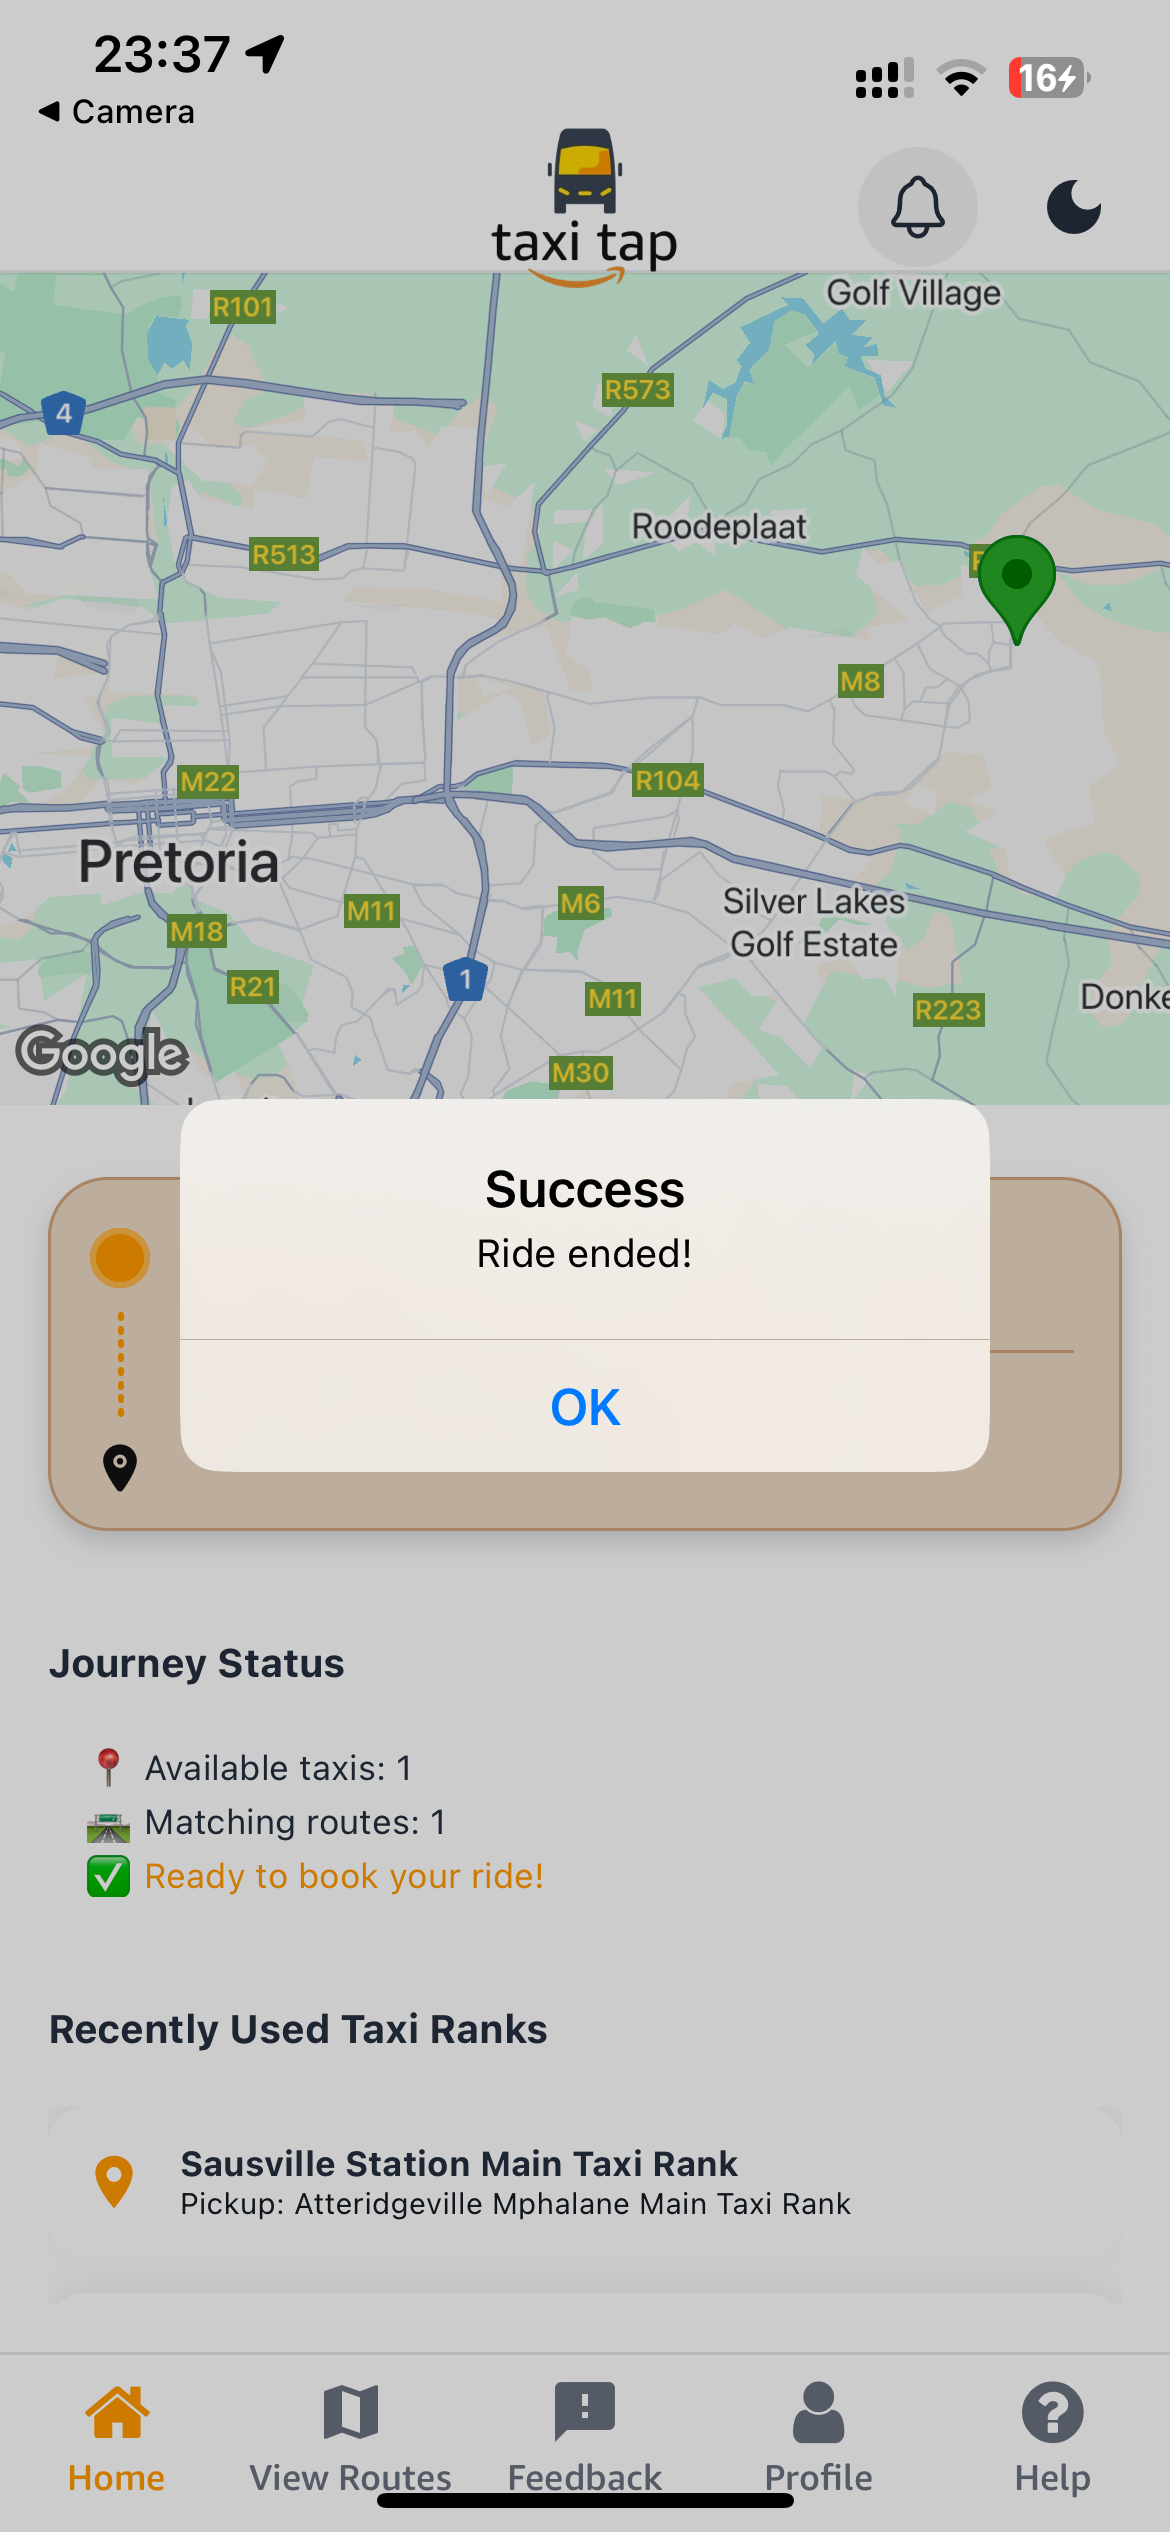
\includegraphics[width=0.4\textwidth]{ride_ended.png}
  \caption{Ride Completion}
\end{figure}

\subsection{Cancelling a Ride}

You can cancel your ride request at any time before the driver accepts it:
\begin{itemize}
    \item Click "Cancel Request" on the ride tracking screen
    \item You'll receive a "Success - Ride cancelled" confirmation
    \item The app will return to the main screen
\end{itemize}

\begin{figure}[H]
  \centering
  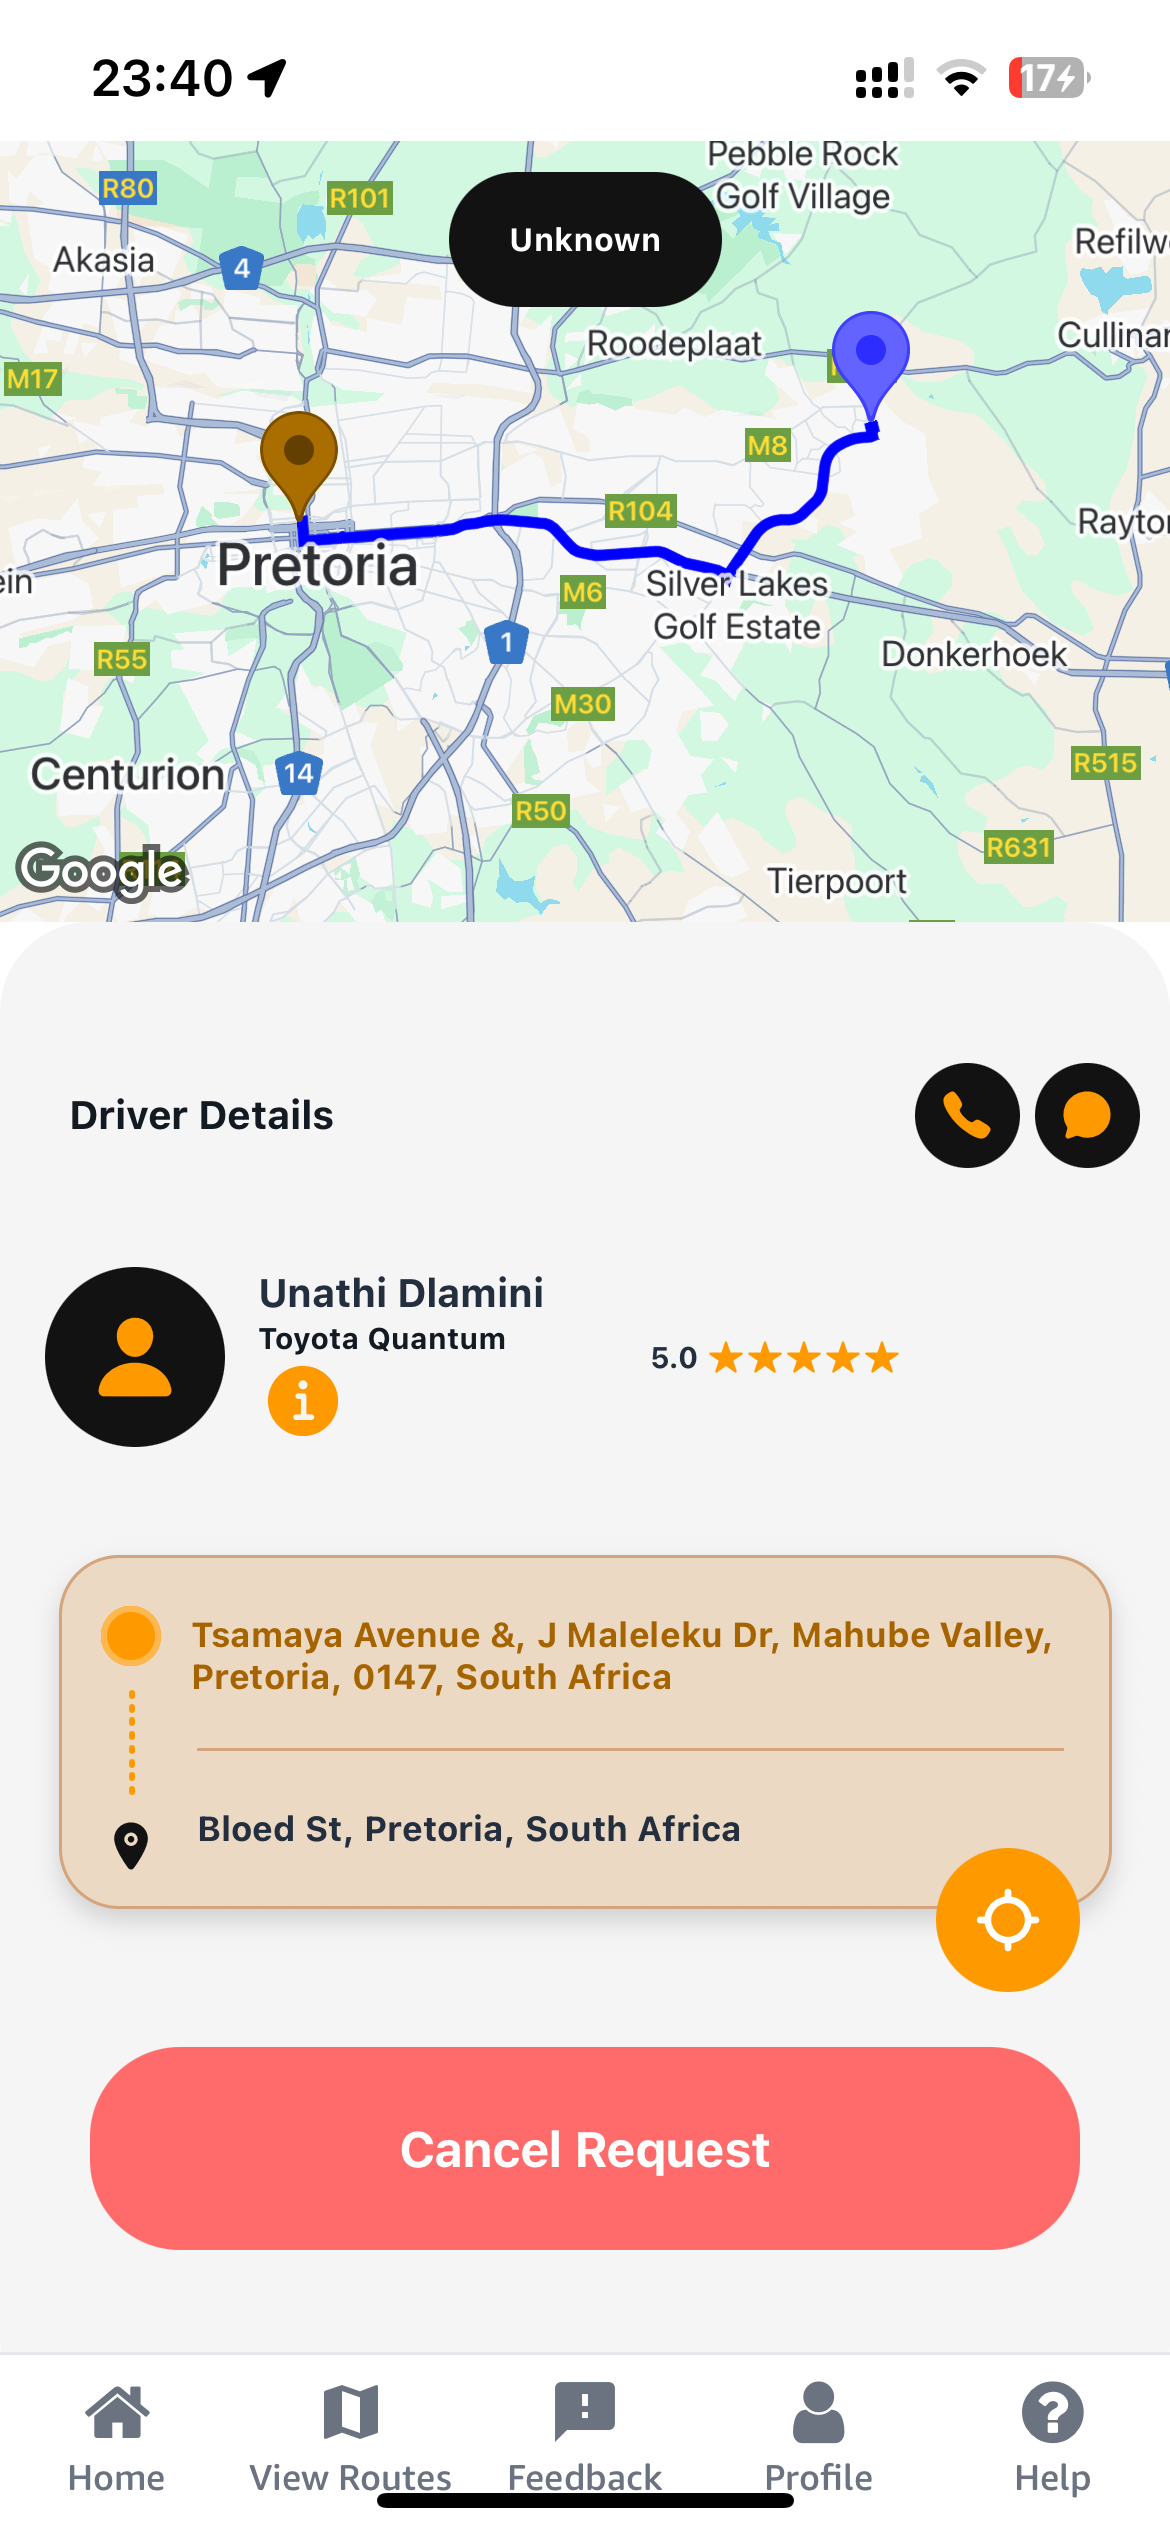
\includegraphics[width=0.4\textwidth]{cancel_request.png}
  \caption{Cancel Request}
\end{figure}

\begin{figure}[H]
  \centering
  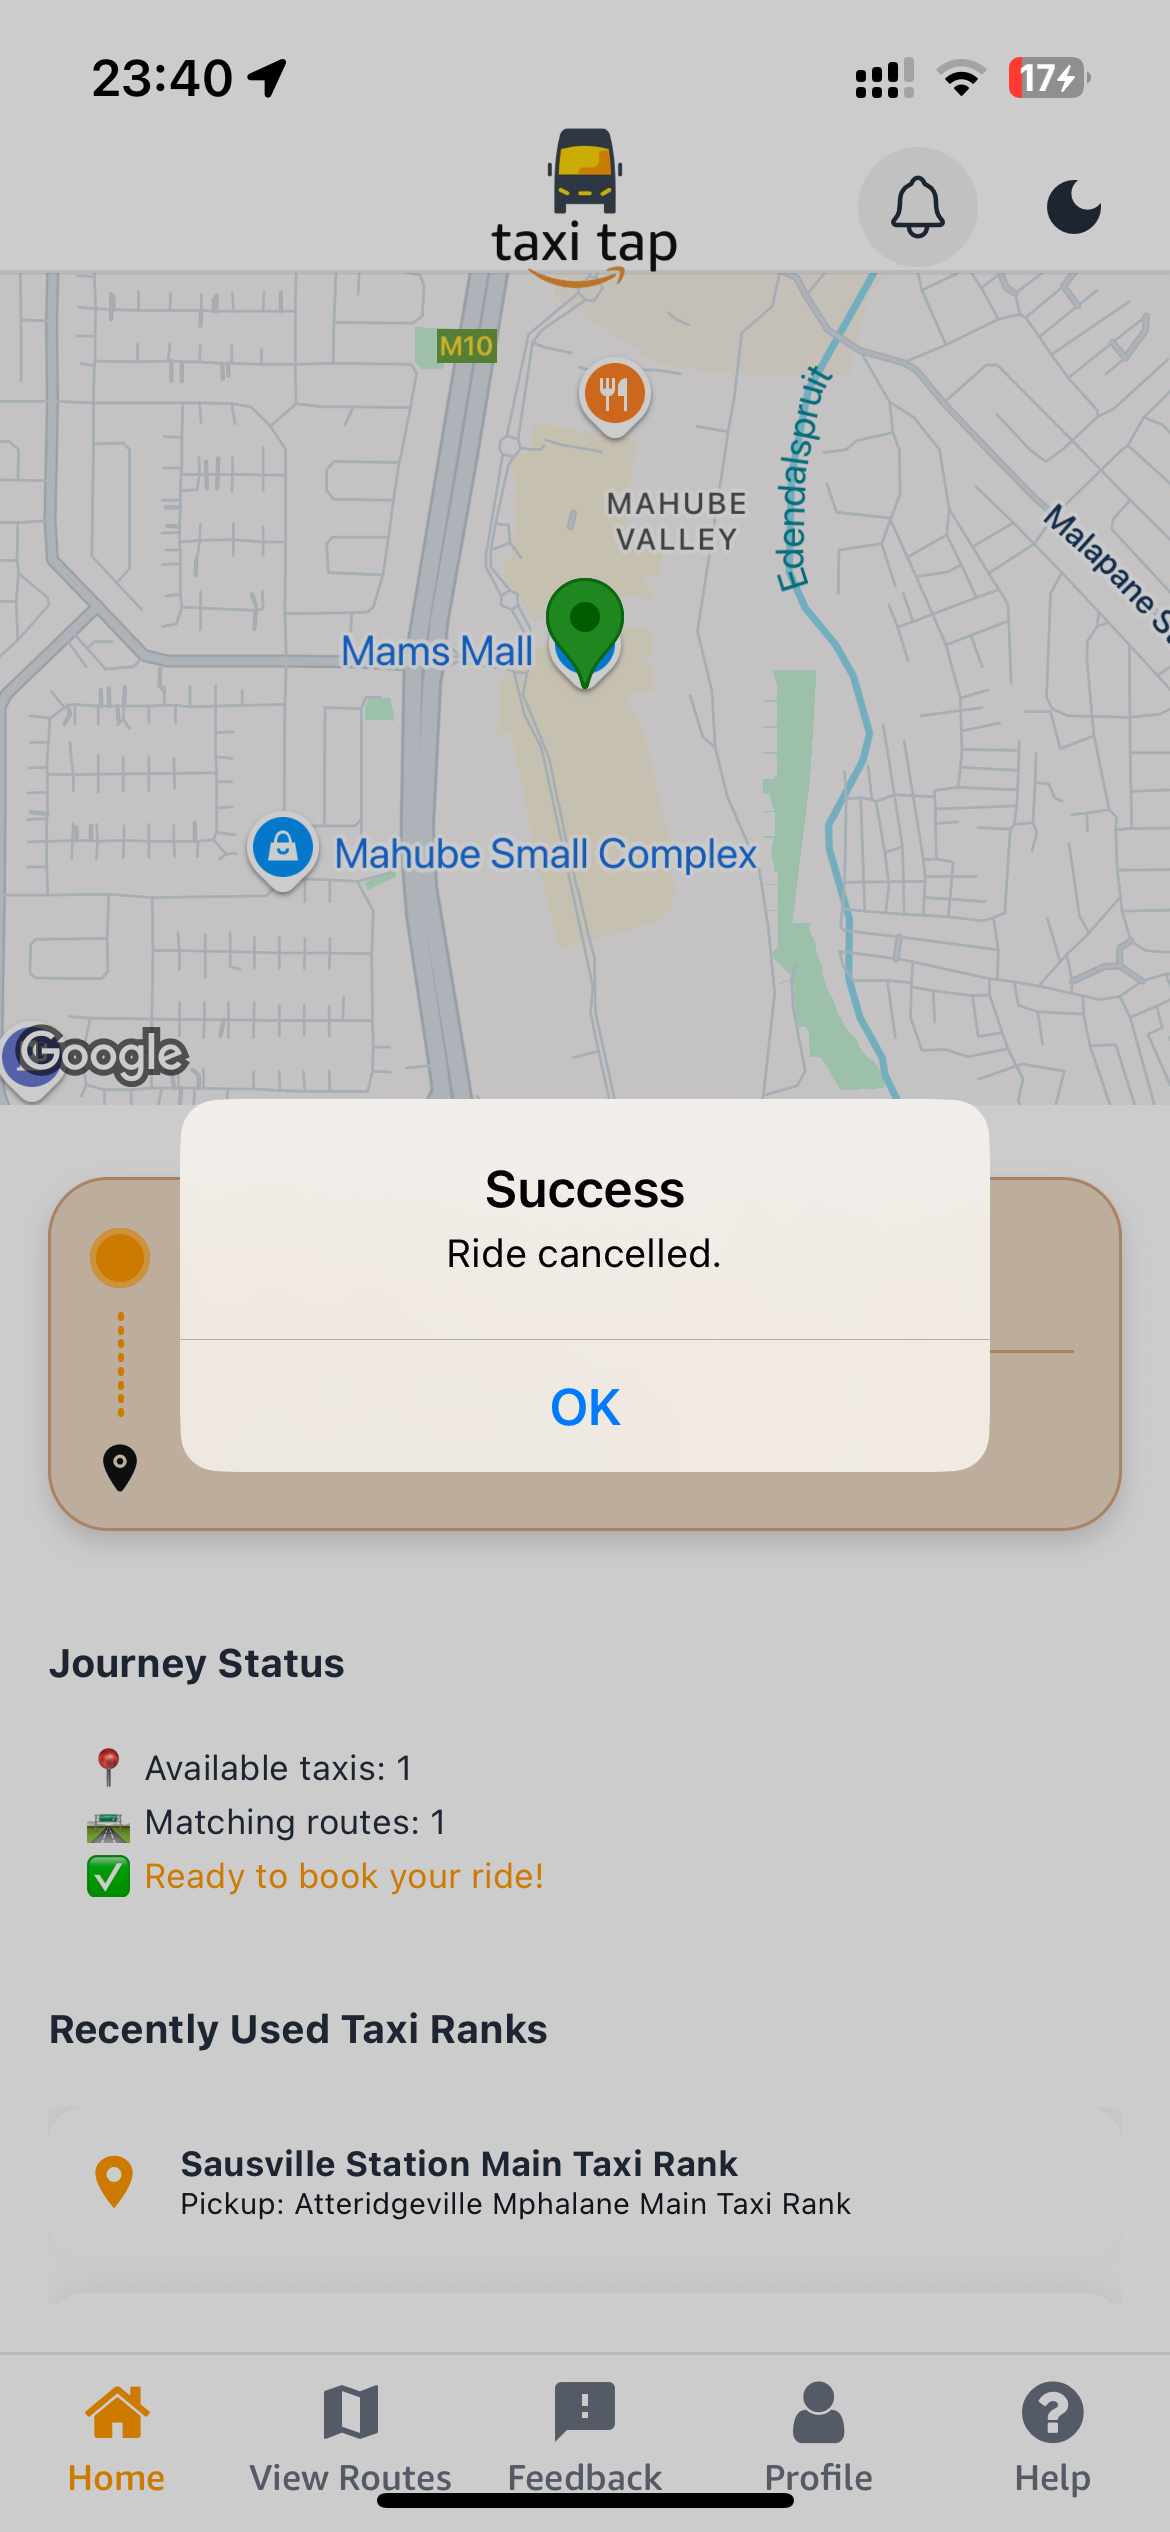
\includegraphics[width=0.4\textwidth]{ride_cancelled.png}
  \caption{Ride Cancellation}
\end{figure}

\section{Driver Interface}

\subsection{Overview}
The Driver interface allows registered drivers to:
\begin{itemize}
    \item Receive ride requests from passengers
    \item Accept or decline requests
    \item Navigate to pickup and drop-off locations
    \item Manage their availability status
    \item Track earnings and ride history
\end{itemize}

\begin{figure}[H]
  \centering
  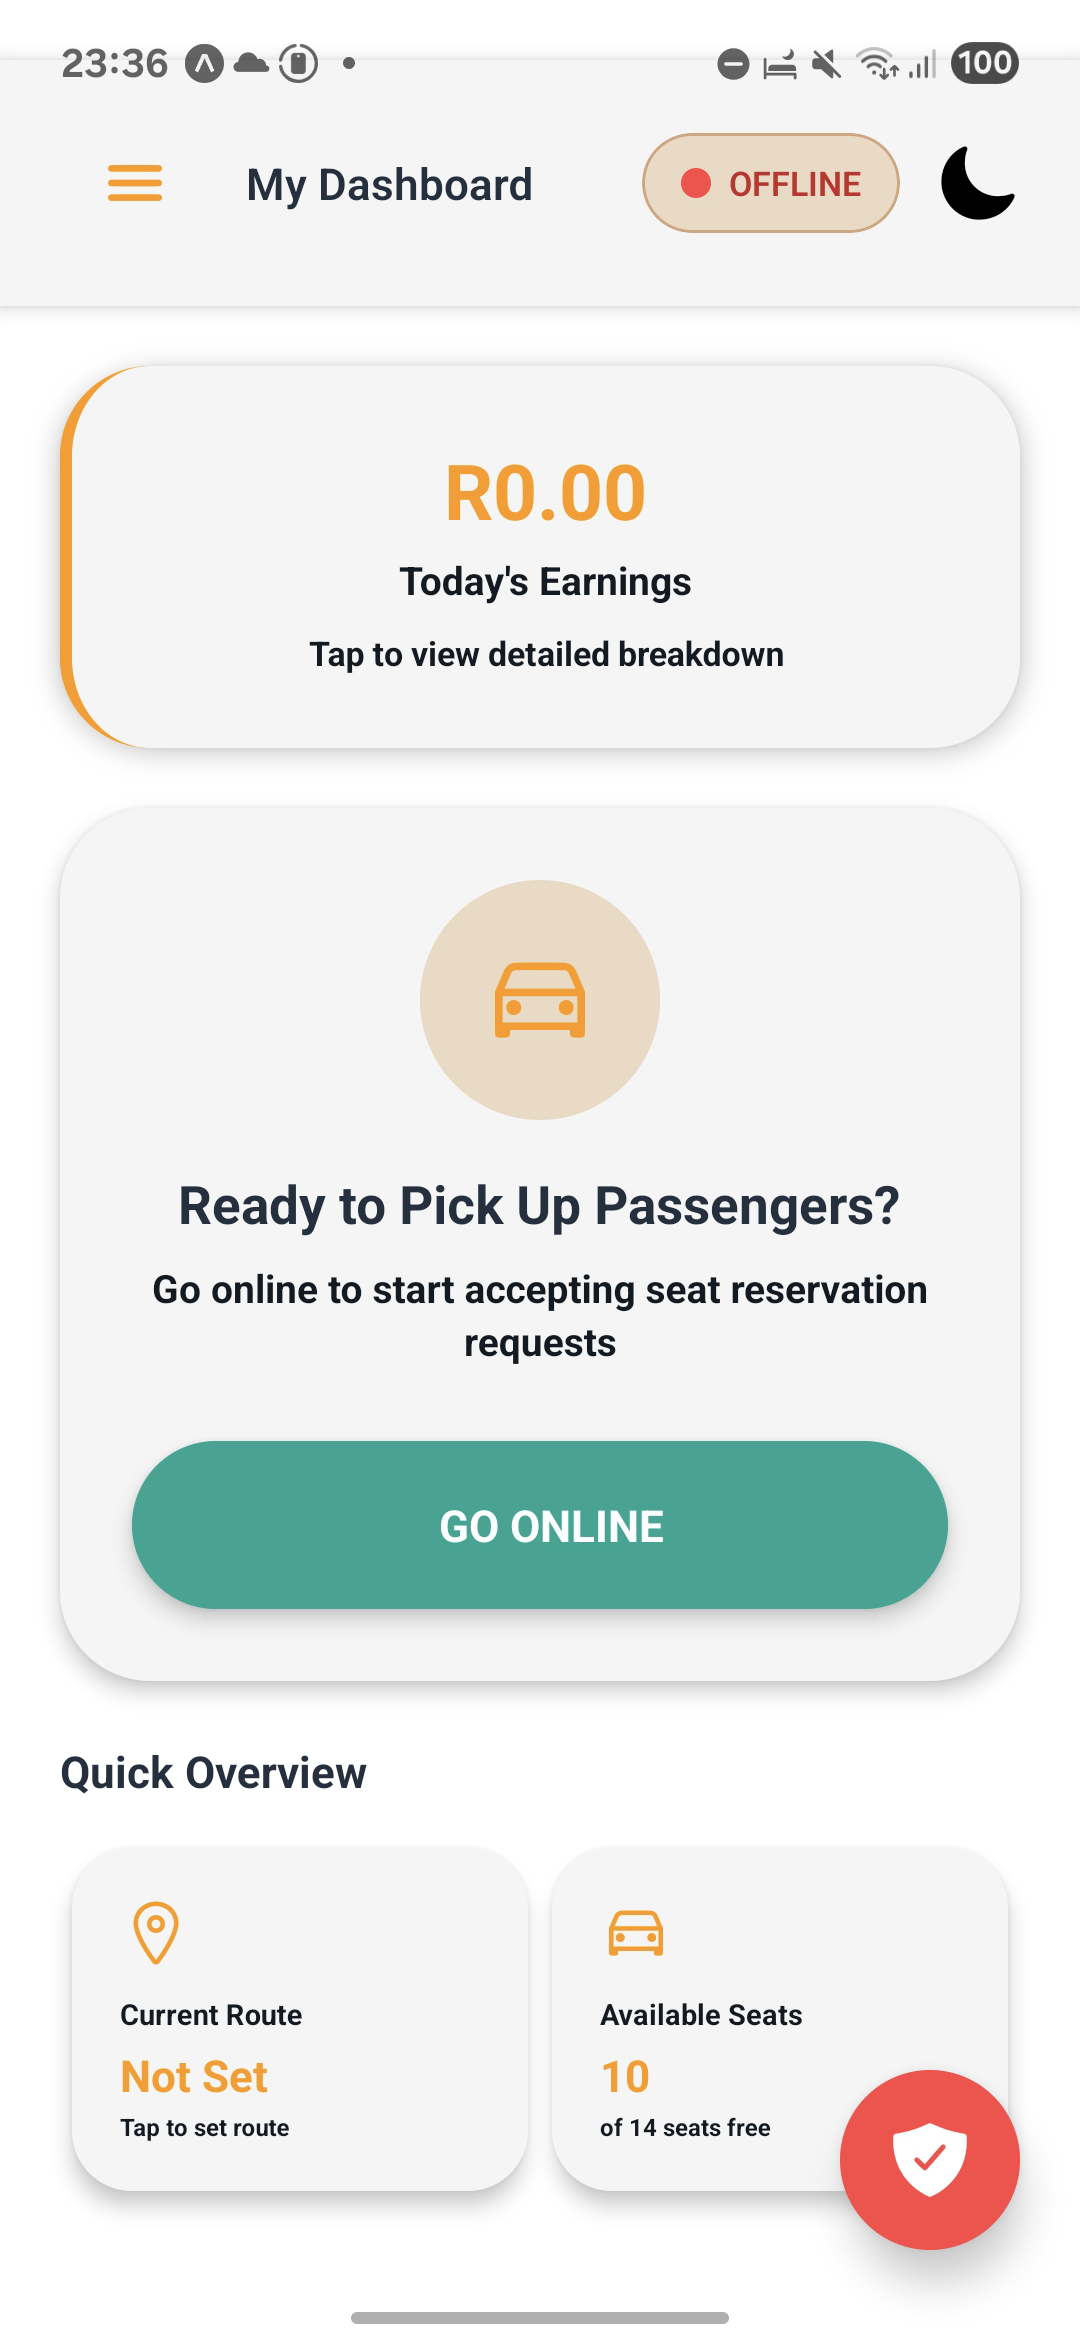
\includegraphics[width=0.4\textwidth]{driver_interface.png}
  \caption{Driver Main Interface}
\end{figure}

\begin{figure}[H]
  \centering
  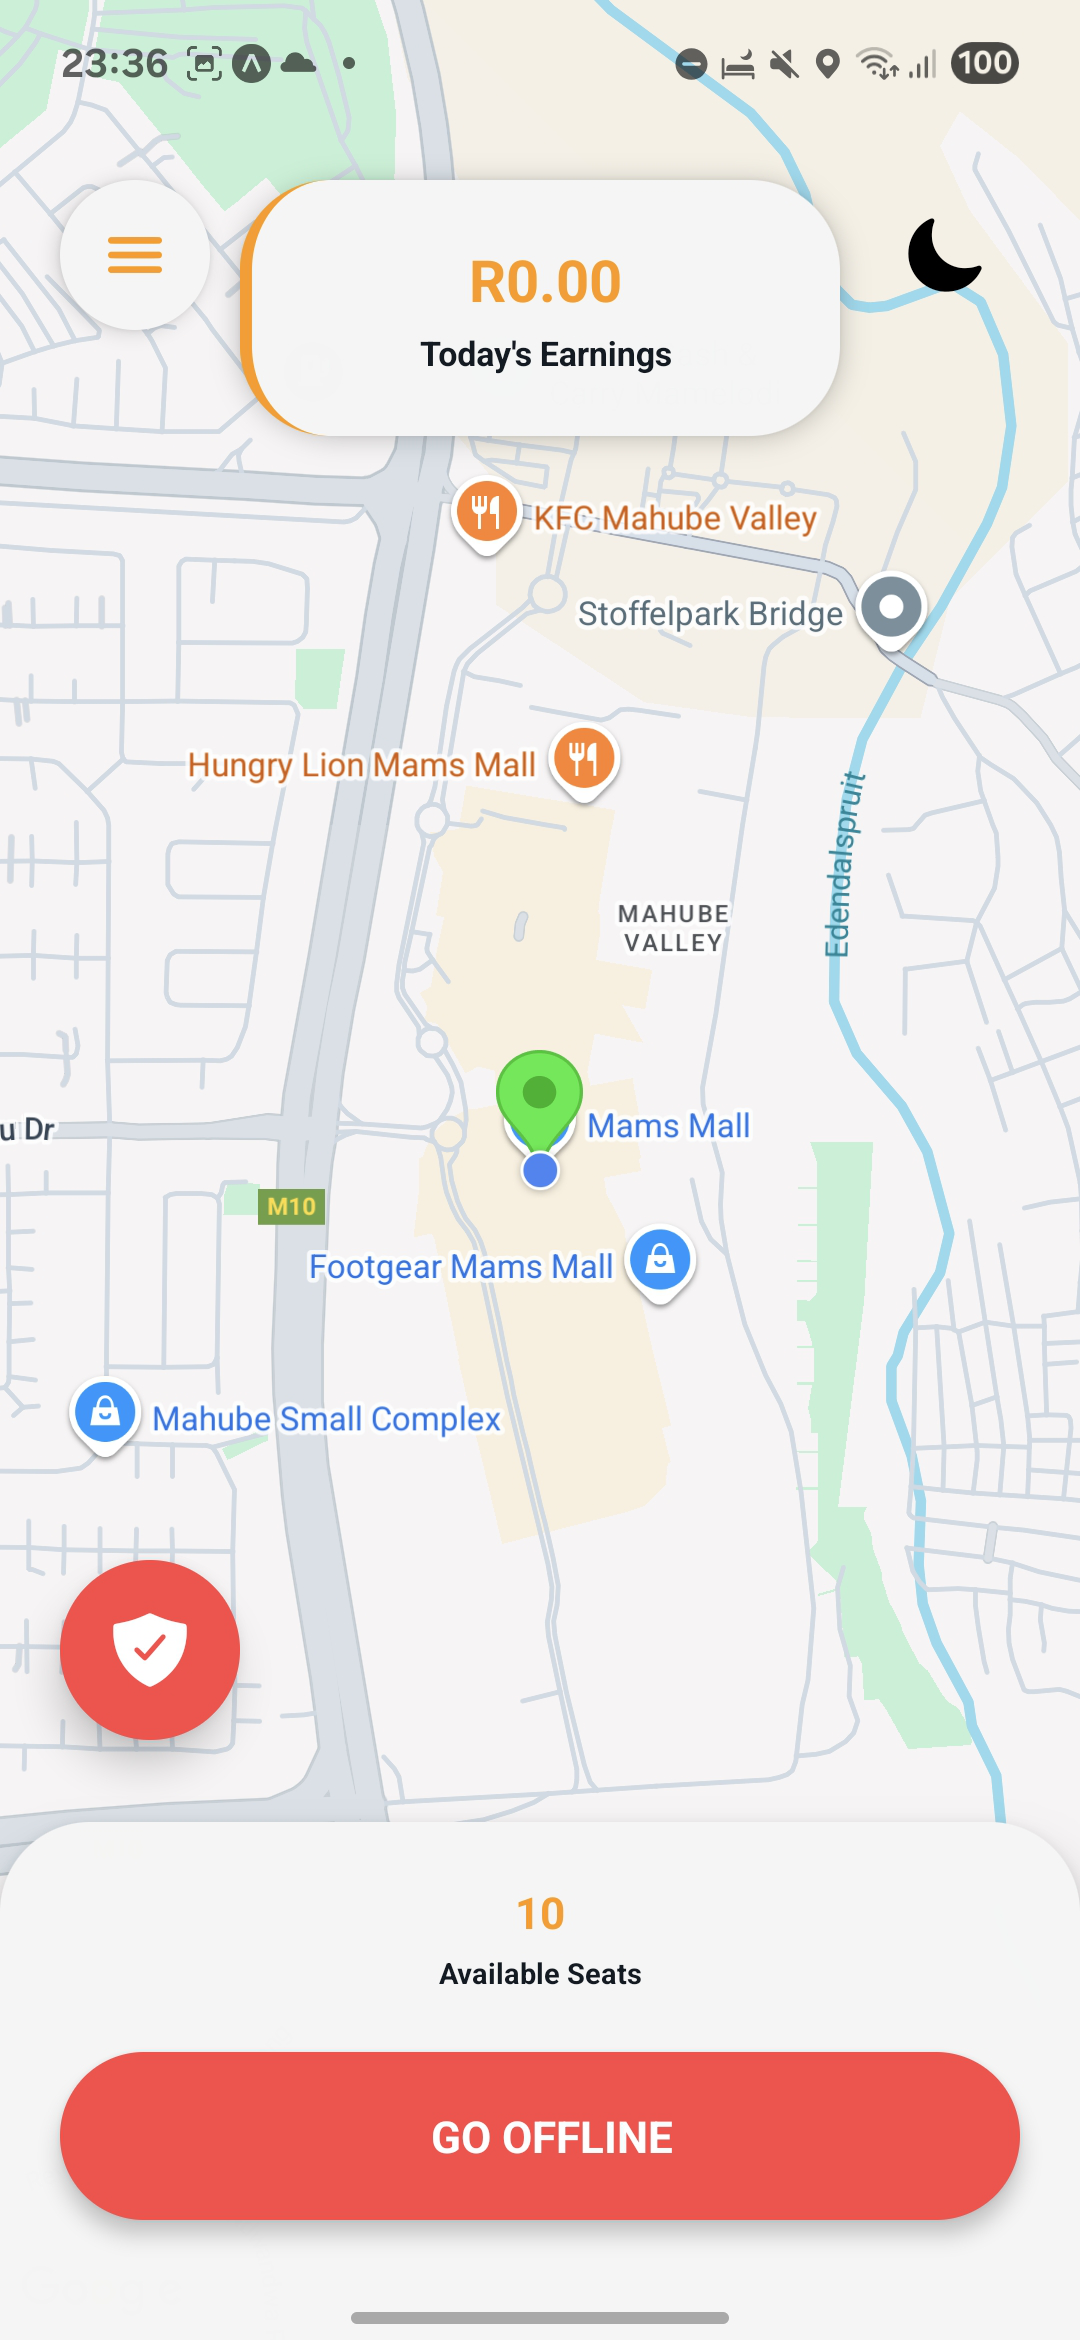
\includegraphics[width=0.4\textwidth]{driver_online.png}
  \caption{Driver Online Interface}
\end{figure}

\subsection{Managing Ride Requests}
\subsubsection{Receiving Requests}
When a passenger requests a ride:
\begin{itemize}
    \item You'll receive a notification with passenger details
    \item The request will show pickup and drop-off locations
    \item You can see the estimated fare and duration
    \item You have the option to accept or decline
\end{itemize}

\subsubsection{Accepting Rides}
To accept a ride request:
\begin{itemize}
    \item Review the trip details
    \item Tap "Accept Ride" if you want to take the request
    \item Navigate to the passenger's pickup location
    \item Confirm pickup when the passenger boards
\end{itemize}

\begin{figure}[H]
  \centering
  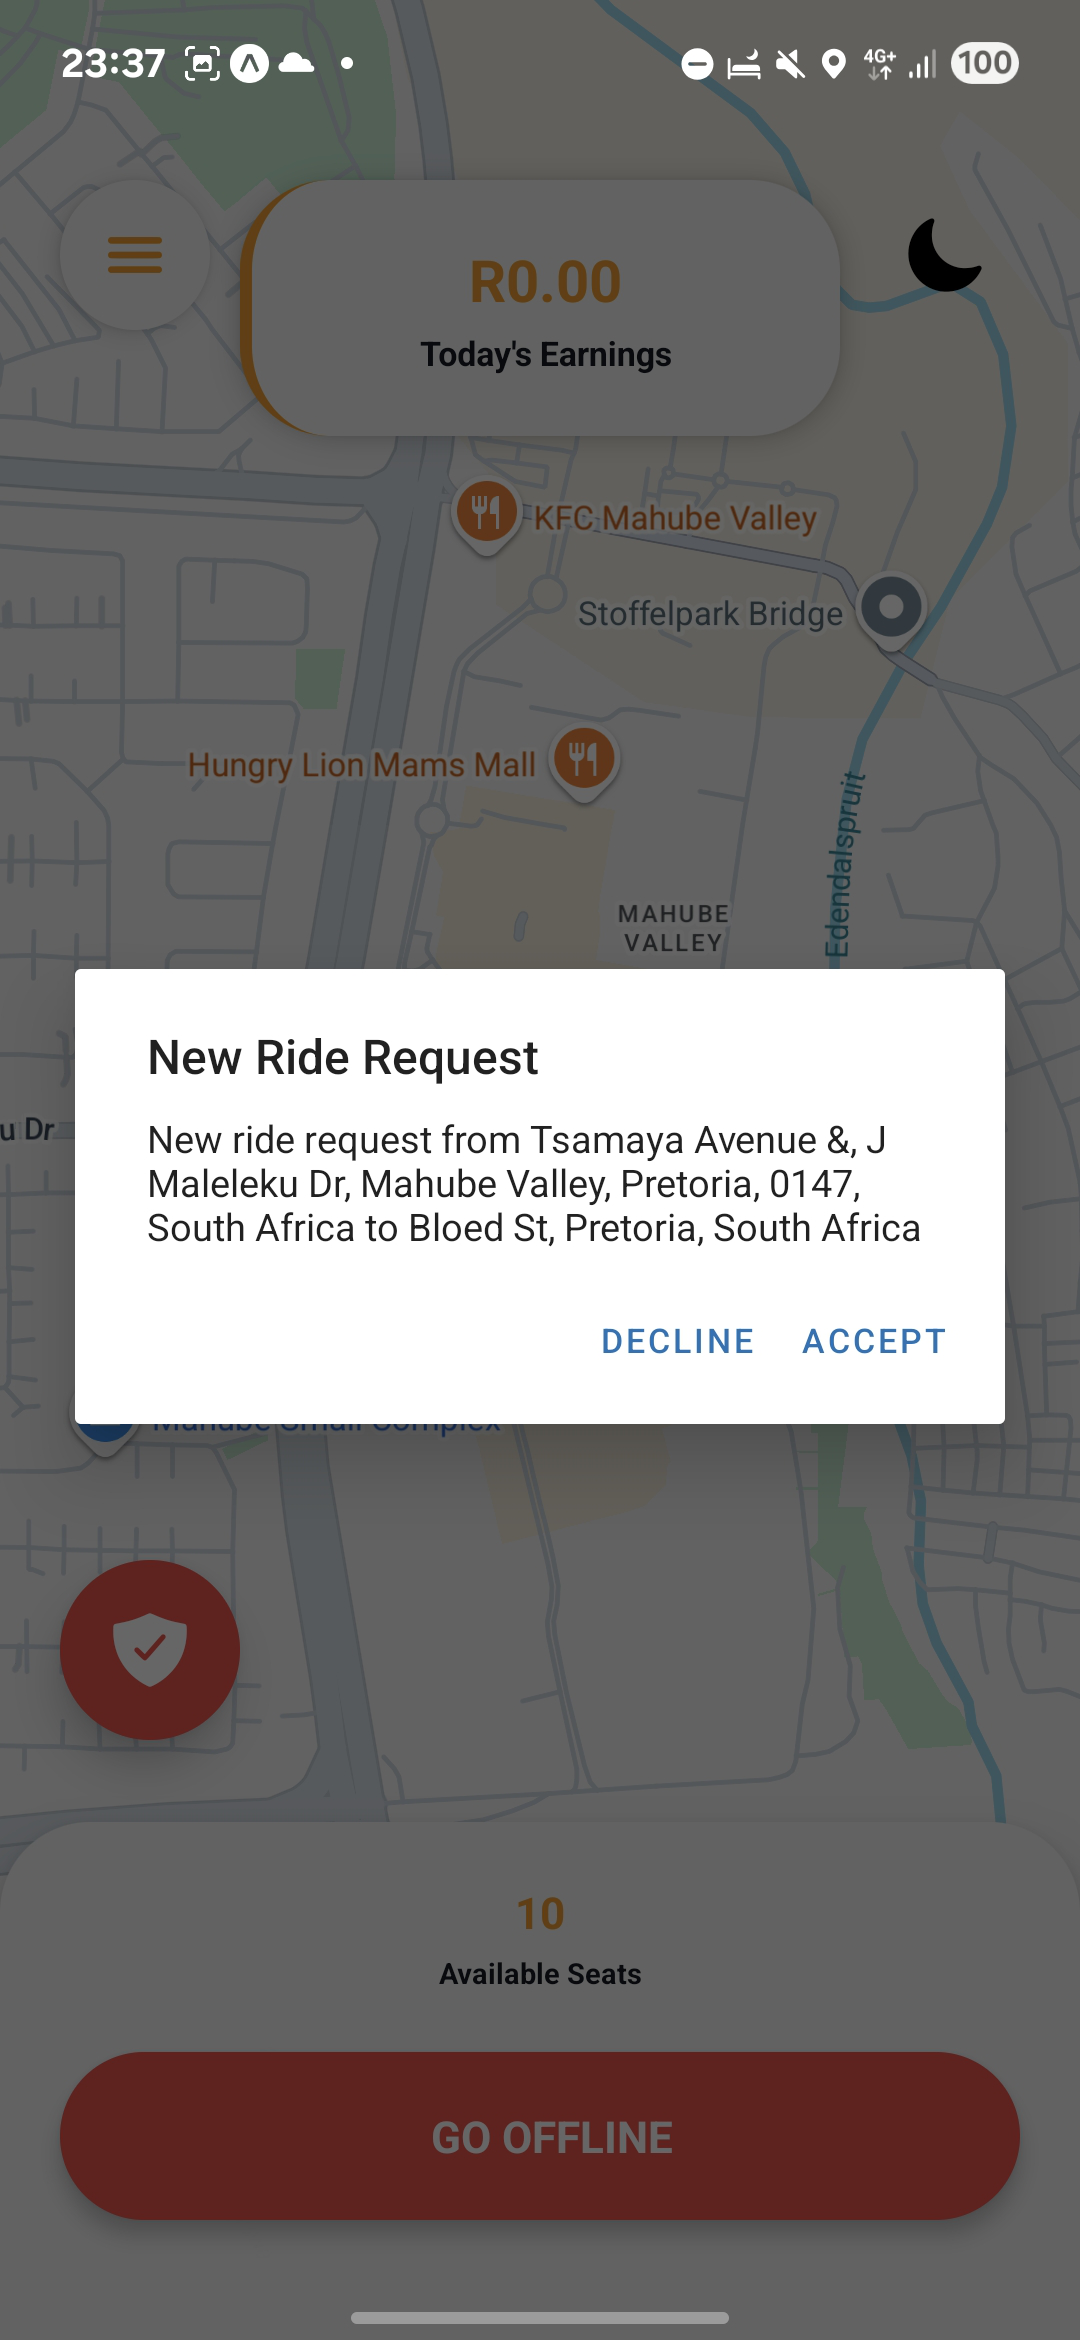
\includegraphics[width=0.4\textwidth]{accept_ride.png}
  \caption{Driver Online Interface}
\end{figure}

\section{Additional Features}

\subsection{Navigation Features}
\begin{itemize}
    \item View Routes: Access detailed route information
    \item Real-time GPS tracking
    \item Turn-by-turn navigation
    \item Alternative routes
\end{itemize}

\subsection{Support and Feedback}
\begin{itemize}
    \item Feedback: Submit feedback about your experience
    \item Help: Access user guides and FAQs
    \item Profile: Manage your account settings
\end{itemize}

\subsection{Recently Used Taxi Ranks}
The app keeps track of frequently used taxi ranks for quick access:
\begin{itemize}
    \item Sausville Station Main Taxi Rank
    \item Atteridgeville Mphalane Main Taxi Rank
    \item Other commonly used pickup points
\end{itemize}

\section{Troubleshooting}

\subsection{Common Issues}
\subsubsection{No Available Taxis}
If no taxis are available:
\begin{itemize}
    \item Check if your location is within the service area
    \item Try requesting again after a few minutes
    \item Consider alternative pickup locations nearby
\end{itemize}

\subsubsection{Connection Issues}
If you experience connectivity problems:
\begin{itemize}
    \item Ensure you have a stable internet connection
    \item Check your GPS settings are enabled
    \item Restart the app if necessary
\end{itemize}


\section{Safety Guidelines}

\subsection{For Passengers}
\begin{itemize}
    \item Verify driver and vehicle details before boarding
    \item Share your trip details with trusted contacts
    \item Use in-app emergency features when needed
    \item Rate your experience to help maintain service quality
\end{itemize}

\subsection{For Drivers}
\begin{itemize}
    \item Maintain vehicle safety standards
    \item Verify passenger identity before pickup
    \item Follow designated routes and traffic laws
    \item Report any safety concerns immediately
\end{itemize}

\section{Contact Information}

For technical support, feedback, or general inquiries:
\begin{itemize}
    \item Email: \href{mailto:gititdone.2025@gmail.com}{gititdone.2025@gmail.com}\\
    \item Website: \url{http://www.gititdone2025.site}
\end{itemize}

Developed by Git It Done Team

\end{document}